\documentclass[msc, cs, deptreport, singlespacing, twoside]{infthesis}
\usepackage{listings}
\usepackage{color}
\usepackage{geometry}
\usepackage{graphicx}
\usepackage{float}
\usepackage{subfig}
\usepackage{array}
\usepackage{textcomp}
\usepackage[colorlinks=true, citecolor=black, linkcolor=black, urlcolor=black, bookmarks]{hyperref}
 
\definecolor{javared}{rgb}{0.6,0,0} % for strings
\definecolor{javagreen}{rgb}{0.25,0.5,0.35} % comments
\definecolor{javapurple}{rgb}{0.5,0,0.35} % keywords
\definecolor{javadocblue}{rgb}{0.25,0.35,0.75} % javadoc

\lstset{
	language=Java,
	basicstyle=\footnotesize\ttfamily,
	keywordstyle=\color{javapurple}\bfseries,
	stringstyle=\color{javared},
	commentstyle=\color{javagreen},
	morecomment=[s][\color{javadocblue}]{/**}{*/},
	numbers=left,
	frame=single,
	numberstyle=\tiny\color{black},
	stepnumber=1,
	numbersep=10pt,
	tabsize=2,
	showspaces=false,
	showstringspaces=false
}


\title{Radio Frequency Localisation/Tracking of RFID Tags in a Raspberry-Pi Sensor Network}
\author{Aleksandar Krastev}

\abstract{
To Do
}

\begin{document}
\begin{preliminary}
\maketitle
\begin{acknowledgements}
To Do
\end{acknowledgements}
\standarddeclaration
\tableofcontents
\end{preliminary}

\chapter{Introduction}
\label{ch:introduction}

\section{Motivation}

\textbf{Copied from IRP}

Radio Frequency Identification (RFID) is an identification technology that also enables tracking of people and objects. RFID functions by remotely obtaining data stored on RFID tags. This information is mainly used for identification purposes. Systems relying on such data can only provide course-grained location information \cite{Bouet2008}. Their RFID readers are positioned at strategic control points in order to recognise tags that enter their read range. However, if an object's identity is combined with its location, then the benefits of RFID could be greater. For example, patient care and hospital operations could be improved using remote identification and tracking of patients \cite{Cangialosi2007}.

RFID localisation principles are similar to the ones used for indoor wireless networks \cite{Bouet2008}. There are certain differences between both technologies, which results in tracking methods that are altered to reflect the characteristics of RFID. This project uses some of these indoor localisation schemes to detect and track a tag using three reader nodes in a controlled indoor environment. 

RFID systems mainly consist of tags and readers. While tags are simple devices, readers are more complex and usually require a connection to a host computer or network \cite{Landt2005}. The high costs of tags and readers are a major factor that constrains the penetration of this technology \cite{Want2006}. Nowadays, these devices are becoming affordable to users . In addition, the recent emergence of cheap and compact single-board computers, such as the Raspberry Pi\footnote{About the Raspberry Pi - \url{http://www.raspberrypi.org/about}}, creates an exiting opportunity to build a cost-effective RFID sensor network capable of localising tags. This can be realised by connecting readers to single-board computers through USB or wired using a breadboard\footnote{Breadboard is a solderless (plug-in) construction base used for experimenting with circuit design.} and general purpose input/output (GPIO) pins on a chip.

On the one hand, the RFID technology has unprecedented advantages and it has gained the attention of big industries that have identified its potential. On the other hand, the high costs of RFID tracking systems and components prevent most people from using and developing the technology. The hardware combination of affordable readers, tags, and single-board computers has the potential to benefit a vast range of businesses but also do-it-yourself hobbyists and enthusiasts. This might result into improved automated handling and tracking of goods in a warehouse, for instance. It can also result in a fast-paced, community-based, and open-source development of the RFID technology applied in a wide range of scenarios. This  project is interesting and exciting because it will try to apply RFID localisation algorithms on affordable hardware in order to create a tracking system. This will show that there can be cost-effective alternatives to commercial solutions, thus making the technology more accessible to a wider audience.

\section{Hypothesis}

\textbf{Copied from IRP.}

The hypothesis of this project is that existing algorithms for localisation and tracking of active tags can be applied on a cost-effective Raspberry-Pi-based sensor network to achieve a similar performance. More specifically, the purpose of the project is to construct and programme three reader nodes, each consisting of a reader connected to a single-board computer, that cooperate in an indoor environment to estimate the position of a stationary or moving active tag based on the Received Signal Strength Indicator (RSSI) using a localisation method called trilateration.

\section{Contributions}

\section{Thesis Outline}

% The thesis is organised into seven chapters including this chapter. The organisation is as follows:

% \begin{itemize}
% \item \textbf{Chapter \ref{ch:background}} gives a background perspective of the concepts and terminologies used throughout this thesis. The anatomy and physiology of the human retina, Gestalt psychology, and the silicon retina are some of the concepts which are discussed.
% \item \textbf{Chapter \ref{ch:related_work}} provides a quick overview of the prior work, which is correlated in some way with the current project. It also explains how the related work helped in designing and implementing the system created by this project. 
% \item \textbf{Chapter \ref{ch:design}} discusses the motivation for the design of the system. It describes issues with the input data from the dynamic vision sensor and how these influenced specific design decisions. Then it gives an insight of how different part of the system work together.
% \item \textbf{Chapter \ref{ch:implementation}} presents a detailed explanations of how the implementation of the system was realised. It gives an insight into the various development stages the implementation has gone through before reaching its final design. It also explains specific details about how different algorithms work.
% \item \textbf{Chapter \ref{ch:results}} presents the methodologies and setup for conducting a number of experiments to test how well different levels of the system performed. It also evaluates the results from those experiments. A discussion of strength and weaknesses of the system is also provided. Possible improvements are suggested as well.
% \item \textbf{Chapter \ref{ch:conclusion}} finally concludes the thesis by presenting the contributions, discussing the difficulties encountered during the project, and suggesting future work.
% \end{itemize}

\section{Summary}

\chapter{Background}
\label{ch:background}

\cite{Want2006}

\section{Summary}

\chapter{Methodology}
\label{ch:methodology}

This project explores the possibility of developing an RFID location sensing system using cost-effective hardware. This chapter gives the reader a detailed overview of the system components and approach to the problem. Section \ref{sec:hardset} presents the hardware setup of the system. Section \ref{sec:probdef} describes the problem this project is trying to solve. Then, the overall software architecture is discussed in section \ref{sec:softarch}. Section \ref{sec:rssitodist} details the methods for converting RSSI to distance measurements. Finally, section \ref{sec:trilatmeth} describes trilateration, a mathematical technique that computes the relative position of an unknown object to three reference objects.

\section{Hardware Setup}
\label{sec:hardset}

The devices used in this project were connected together to form the hardware setup of the system. These components and their specifications are described in detail in section \ref{sec:projhard}. Figure \ref{fig:hardset} is a diagram illustrating how the hardware devices were attached to each other.

\begin{figure}[h]
	\begin{center}
		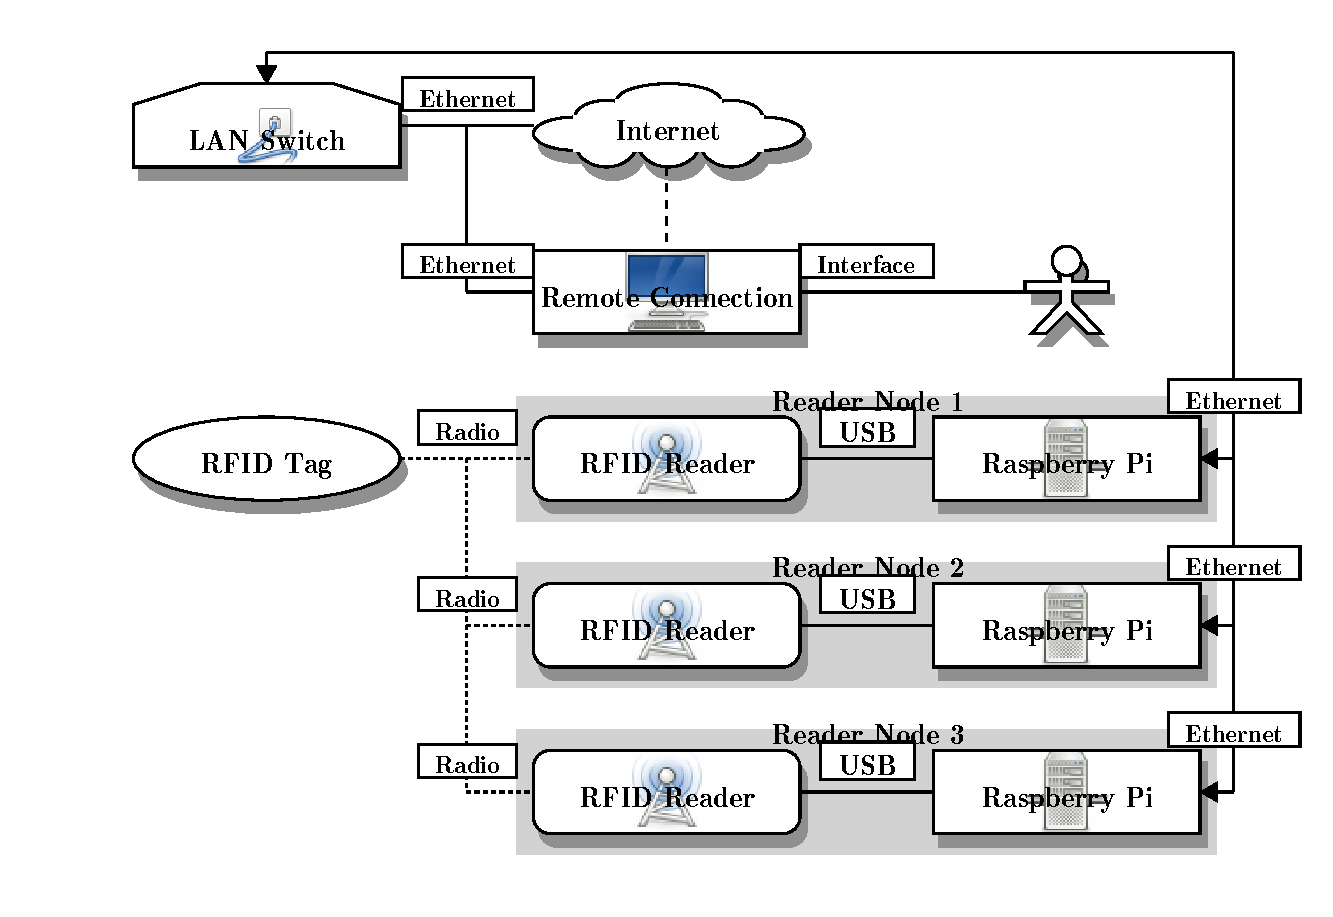
\includegraphics[width=1\textwidth]{figures/blockdiag/hardwaredesign}
		\caption{Hardware setup of the project.}
		\label{fig:hardset}
	\end{center}
\end{figure}

\subsection{Reader nodes}

The building blocks of the system are the reader nodes. Each consists of an RFID reader connected to a Raspberry Pi using USB. The project plan had provisioned extra time to account for the possible complications when interfacing between serial devices and single-board computers. The Raspberry Pis have USB ports that cannot power all kinds of USB devices. Another issue was whether the computers were capable of recognising and communicating with these specific RFID readers. Fortunately, these potential problems did not occur during this project. The RFID devices read identification data from the RFID tag over the air.

\subsection{Computer Network}

The Raspberry Pis were connected in a local area computer network (LAN) using Ethernet cables and a network switch. This allowed them to communicate readings to each other. The Raspberry Pi network provided means for remotely accessing, programming, and controlling the reader nodes. Remote access was established by connecting to the network using the network switch or through a wide area network, such as the Internet.


\subsection{Alternative connectivity using Wi-Fi}

During the project planning phase, an alternative connectivity method was considered. The Raspberry Pis have two USB ports. One of them was occupied by a RFID reader. The spare one could have been used for a wireless network adapter. Then, all reader nodes could connect to a wireless router or form an ad hoc network in order to communicate measurements. This way all Ethernet cabling and the network switch are not required giving a greater flexibility when positioning the reader nodes. Figure \ref{fig:hardsetwifi} in Appendix \ref{sec:hardsetwifi} shows this alternative hardware setup.

There are two matters that complicate this choice of connectivity. First, there is a high probability that the power fed to the USB ports is not enough to supply both an RFID reader and a Wi-Fi adapter. In which case, three powered USB hubs were needed to be purchased. Second, the Raspberry Pis have integrated Ethernet ports. Buying three wireless USB dongles is an unjustifiable expense in case these might not get powered by the single-board computers.

\section{Problem Definition}
\label{sec:probdef}

Given the hardware setup of the system consisting of three reader nodes connected into a computer network, the problem it is trying to solve is to estimate the relative position of an RFID tag to three RFID readers. The system should accept the following inputs:
\begin{itemize}
	\item identification information received from the RFID tag,
	\item RSSI measurements computed at the RFID readers,
	\item and positions of the reader nodes in three dimensions.
\end{itemize}
The system should output the location of the RFID tag relative to the reader nodes. The system should be able to estimate the tag's position when it is:

\begin{itemize}
 	\item stationary,
 	\item in motion,
 	\item unobstructed from any objects,
 	\item occluded by a single or multiple objects. 
\end{itemize}
 
Combinations of the above cases provide a basis for experiments to check whether the problem is solved by the system. To determine how well the system performs, the accuracy of localisation is compared to previous systems described in section \ref{sec:prevwork}.

\section{Software Architecture}
\label{sec:softarch}

The system consists of three network nodes that need to aggregate reader measurements on a single computer in order to process the data. A server-client model was chosen because the measurements are collected in one place, which is convenient for converting RSSI values to distance and computing the tag's position. Figure \ref{fig:sercli} shows a conceptual diagram of the server-client model used in this project. Every Raspberry Pi is capable of being both a server and a client. A disadvantage of this model is the single point of failure of the system. If the server fails, then another node needs to become an aggregator of data otherwise the system would not function as intended.

\begin{figure}[h]
	\begin{center}
		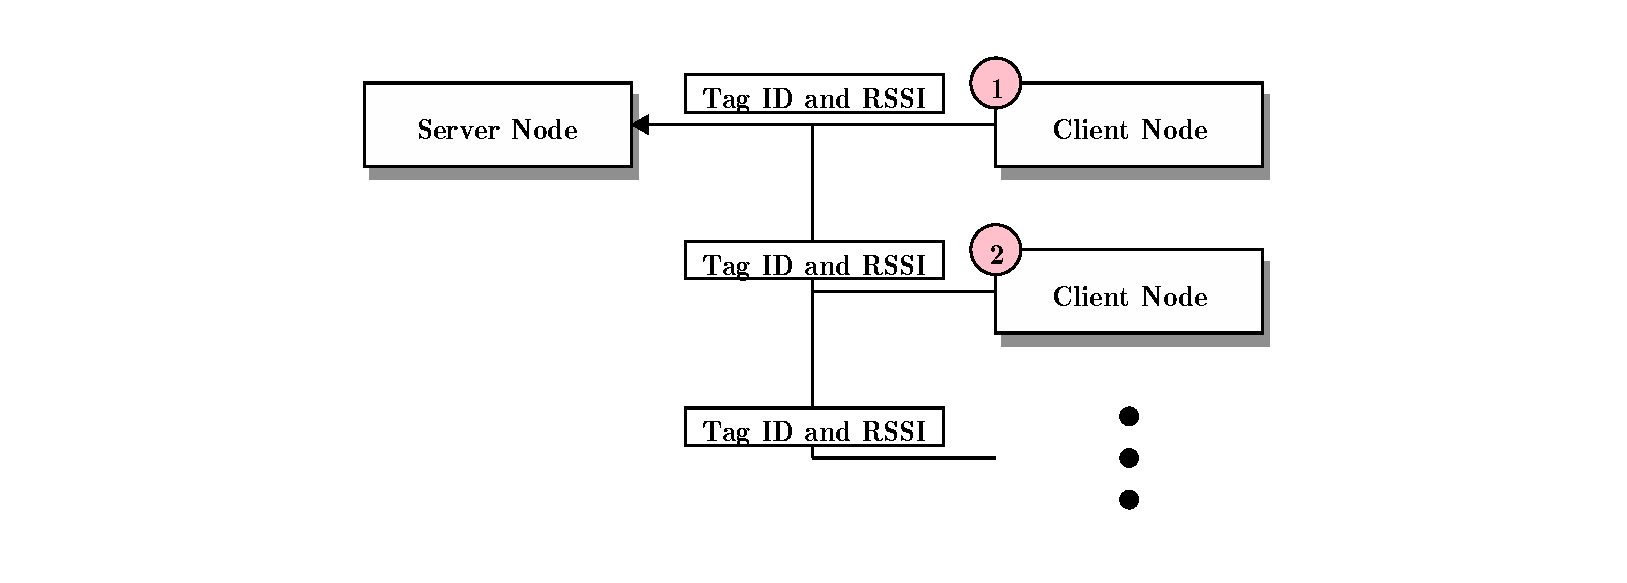
\includegraphics[width=1\textwidth]{figures/blockdiag/serverclient}
		\caption{Conceptual diagram of the server-client model.}
		\label{fig:sercli}
	\end{center}
\end{figure}

Client nodes have two main responsibilities. First, they read the identity and RSSI of the tag. Second, clients send this data on the network to the server. A server node provides the following functionality. It receives measurements from other nodes. A server also reads the tag's identity and RSSI. Then, this computer converts the RSSI values into distance. Distance measurements together with the positions of the reader nodes are input into a localisation algorithm. These steps are illustrated on Figure \ref{fig:sercliresp}.

\begin{figure}[h]
	\begin{center}
		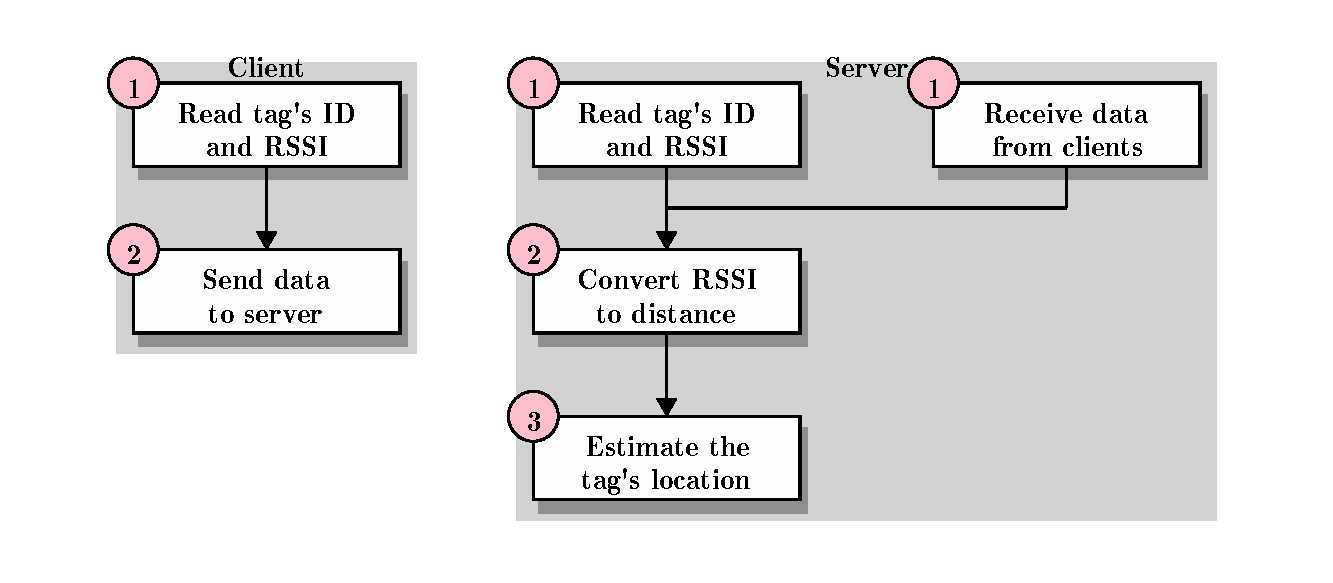
\includegraphics[width=1\textwidth]{figures/blockdiag/serverclientresp}
		\caption{Diagram of the general server and client responsibilities.}
		\label{fig:sercliresp}
	\end{center}
\end{figure}

\section{Converting RSSI to distance}
\label{sec:rssitodist}

One of the main challenges of this project was to find a reliable way of converting RSSI values into distance from RFID readers to a tag. As discussed in Section \ref{subsec:rsssianddist}, studies have shown that RSSI is not a reliable or accurate measure of distance. Nevertheless, RSSI is one of the main parameters of this system and distance estimation is solely based on it.

\subsection{Free-space Path Loss}

The first attempt to provide a conversion between RSSI and distance was relying on the inverse-square physical law and free-space path loss (FSPL) formula. In free space propagation, electromagnetic waves obey the inverse-square law stating that the intensity of the emitted radiation is inversely proportional to the square of the distance from the source of the emitted radiation \cite[p. 19]{Schlaikjer1962}. This can be expressed as the following relation:

\[ Intensity \propto \frac{1}{distance^{2}} \]

A more complete relationship between signal strength and distance is given by the FSPL formulation. Free-space path loss is the loss in signal strength of an electromagnetic wave propagating through free space without any obstacles \cite{Balanis2012}. FSPL is proportional to the square of both distance and frequency of the radio signal. It can be expressed in terms of decibels given distance in meters and radio frequency in megahertz\footnote{Derivation the dB version of the FSPL equation - \url{http://www.ece.uvic.ca/~peterd/35001/ass1a/node1.html}}: 

\[ FSPL(dB) = 20\log_{10}(d_{meters}) + 20\log_{10}(f_{MHz}) - 27.55 \]
	
Rearranging the terms of the equation to find the distance gives:

\[ d_{meters} = 10^{(FSPL(dB) - 20\log_{10}(f_{MHz}) + 27.55) / 20} \]

Section \ref{subsec:rssiandrss} discussed the relationship between RSSI and received signal strength (RSS). RSSI is a unitless measurement derived from the values of the RSS. In Section \ref{subsec:receiver}, Figure \ref{fig:rssi} shows the relationship between RSSI and RSS for the RFID receivers used in this project. Consequently, RSSI values can be converted to received signal strength expressed in $dBm$ and inserted into the equation above as $FSPL(dB)$. The frequency of the RFID project hardware is  $315MHz$ (see Table \ref{tbl:reader} and \ref{tbl:tag}).

There are three problems with this approach. First, it models how the signal strength decreases in a line-of-sight propagation in a free from obstacles environments. This project is concerned with location sensing in indoor spaces making the free-space path loss formula inappropriate for this setting. Second, computing the distance for the minimum ($0dB$) and maximum ($60dB$) values of the signal strength range results in distances $0.075$ and $75.716$ meters, which is beyond the practical range of the RFID devices. Third, the conversion from RSSI to RSS might not be appropriate in this case. The RFID equipment for this project is more affordable compared to commercial RFID equipment\footnote{How much do RFID readers cost today? - \url{http://www.rfidjournal.com/faq/show?86}}. As a result, the online support and specifications are scarce, which raises the question to what extent these can be trusted. Moreover, the manufacturer claims a RSSI resolution of eight bits outputting values between 0 and 255. During the range experiments with this hardware a much smaller resolution was recorded. Consequently, converting RSSI unitless values to received signal strength in $dBm$ cannot be relied upon. For details on the evaluation of the RFID devices refer to \textbf{REF}. 

\subsection{Translation table}

Rather than relying on the physical relationship between electromagnetic waves and distance, a simpler and more direct approach was taken. For each RFID reader, a translation table was constructed mapping RSSI to distance. According to the manufacturer, but also observed in hardware experiments, reader measurements vary between different devices. There are two reasons for this. First, the RFID readers are handmade, which introduces small differences in their circuits. Second, the devices are not calibrated to each other when being built.   

The methodology for constructing these translation tables relies entirely on RSSI measurements collected while evaluating the RFID devices. A number of experiments were conducted testing how RSSI changes as the distance between a reader and tag increases. In order to account for the characteristics of indoor environments, these experiments have taken into account the orientation of the tag to the reader, line-of-sight propagation versus obscuring the tag with an obstacle, and elevation of the tag to the reader. Combining measurements from different experiments gives a more realistic representation of how RSSI changes in an indoor environment. Table \ref{tbl:trans} presents the translation table constructed for the first reader. Similar tables were developed for the other two devices (see Appendix \ref{sec:trans}).

\begin{table}[h]
	\centering
	\begin{tabular}{ | c | c | c || c | c || c | c || c | c || c | c || c | c || c | c | }
		\hline
		Distance 	& 0  & 1  & 1  & 2  & 2  & 3  & 3  & 4  & 4  & 5  & 5  & 6  & 6  & 7  \\ \hline
		RSSI 		& 80 & 65 & 64 & 62 & 61 & 57 & 56 & 53 & 52 & 48 & 47 & 46 & 45 & 44  \\ \hline
	\end{tabular}
	\caption{RSSI value ranges used to estimate distance when using the first reader.}
	\label{tbl:trans}
\end{table}

As an example, the first two columns of Table \ref{tbl:trans} have the following meaning. When the reader and tag antennas were touching the average RSSI value from all experiments was 80. When the tag was one meter away from the reader, the average RSSI value of all experiment measurements was 65. RSSI values between 80 and 65 are linearly converted to the new range from zero to one meters as follows: 

\[Old.range = old.min - old.max \\\]
\[New.value = new.min + (old.min - old.value) / old.range\]

An obvious limitation of these conversions is the size of the RSSI ranges. For example, there are 15 possible values that the first reader could measure when the tag is between zero and one meters away from it. In contrast, for a distance between six and seven meters the RSSI values change only by one unit. Following from that, the granularity of the distance estimation changes depending on the range of the RSSI measurements. This is caused by a hardware limitation of the readers when measuring RSSI and has been found during the range experiments presented in \textbf{REF}.

There is another factor contributing to the accuracy of this conversion. The RFID tag is using a battery for its power supply. During continuous operation the battery power level gradually drops, thus the tag emits a weaker radio signal as the battery is being depleted. This is reflected in the RSSI measurements making the translation tables inaccurate. In order to account for the RSSI changes, the incoming measurements were increased by an integer factor chosen based on observation. Different factors were selected for each reader due to their measurement differences.

In summary, this conversion method is not universal and probably cannot be applied to other brands of RFID devices. There are numerous factors that contribute to the variations in RSSI such as radio signal reflection, multi-path fading, and shadowing, to name a few. Nevertheless, this method was selected to translate RSSI to distance. Once the translation tables are constructed, it is a matter of calibration. As mentioned above, RSSI to distance conversion is one of the main variables of this system. How these translation tables performed is discussed in Section \textbf{REF}, where the evaluation results of the system in terms of localisation accuracy are presented.


\section{Trilateration}
\label{sec:trilatmeth}

Trilateration is a localisation method computing the position of an unknown object based on range measurements from three reference points at known locations. The concept of this technique was described in Section \ref{sec:trilatback}. This section presents the mathematical technique used in this project that provides an exact and computationally efficient solution for three-dimensional position estimation. The solution is based on the work of Manolakis \cite{Manolakis1996} and the Wikipedia article on trilateration \cite{Wikipedi2013}.

\subsection{Special case}

In three-dimensional Cartesian coordinate system, the equations for three spheres are:
\begin{align*}
	r_1^2 &=(x-x_1)^2+(y-y_1)^2+(z-z_1)^2 \\
	r_2^2 &=(x-x_2)^2+(y-y_2)^2+(z-z_2)^2 \\
	r_3^2 &=(x-x_3)^2+(y-y_3)^2+(z-z_3)^2 \\
\end{align*}
where the sphere centres are $\vec p_1 = (x_1, y_1, z_1), \ \vec p_2 = (x_2, y_2, z_2), \ \vec p_3 = (x_3, y_3, z_3)$ and $r_1$, $r_2$, and $r_3$ are the sphere radii. Solving these equations for $x$, $y$, and $z$ would give their intersection point. However, this is hard to do directly. In order to simplify the calculations, a special case is defined that can be later used as the basis for a general solution. There are three requirements of the special case. First, the three centres of the spheres are on the $z=0$ plane, hence working in two dimensions. Second, one of the centres of the spheres, $\vec p_1$, is located at the origin. Third, another sphere centre, $\vec p_2$, is on the $x$-axis, thus two of the spheres are collinear. The equations for the three spheres can be rewritten as follows:
\begin{align}
	r_1^2 & =x^2+y^2+z^2 \label{eq:1}\\
	r_2^2 & =(x-d)^2+y^2+z^2 \label{eq:2}\\
	r_3^2 & =(x-i)^2+(y-j)^2+z^2 \label{eq:3}
\end{align}
where $d$ is the distance between sphere centres $\vec p_1$ and $\vec p_2$ and $i$ and $j$ are the signed magnitudes of the $x$ and $y$ components of the vector from $\vec p_1$ to $\vec p_3$. Figure \ref{fig:trilat2} illustrates these components and the positions of the spheres in the $z=0$ plane.

To solve these equations, first subtract \ref{eq:2} from \ref{eq:1} and solve for $x$:
\[x=\frac{r_1^2-r_2^2+d^2}{2d}\]
Next, subtract \ref{eq:3} from \ref{eq:1} and solve for $y$:
\[y=\frac{r_1^2-r_3^2+i^2+j^2}{2j}-\frac{i}{j}x\]
Finally, use \ref{eq:1} to solve for $z$:
\[z=\pm \sqrt{r_1^2-x^2-y^2}\]
These three equations  provide the coordinates of the intersection point $(x,y,z)$ of the three spheres.

\begin{figure}[h]
	\begin{center}
		\def\svgwidth{0.6\textwidth}
		\input{figures/trilat2.pdf_tex}
		\caption{Figure showing three intersecting spheres in the plane containing their centres. Figure from \cite{Wikipedi2013}.}
		\label{fig:trilat2}
	\end{center}
\end{figure}

\subsection{General solution}

The solution of the aforementioned case cannot be applied in a general three-dimensional case because its requirements are not met. This is overcome by treating the sphere centres, $\vec p_1$, $\vec p_2$, and $\vec p_3$, as vectors from the origin:
\begin{align*}
	\vec p_1 &= (x_1, y_1, z_1) \\
	\vec p_2 &= (x_2, y_2, z_2) = \vec p_1 + \hat e_x d \\
	\vec p_3 &= (x_3, y_3, z_3) = \vec p_1 + \hat e_x i + \hat e_y j \\
\end{align*}
where $\hat e_x$, $\hat e_y$, and $\hat e_z$ are the basis unit vectors in the $x$, $y$, and $z$ original coordinate system; $d$, $i$, and $j$ are the same variables defined above. The unit vectors and variables are expressed as follows:
\begin{align*}
	& d = \| \vec p_2 - \vec p_1 \|, &&  i = \hat e_x \cdot ( \vec p_3 - \vec p_1 ), && j = \hat e_y \cdot ( \vec p_3 - \vec p_1 ) \\
	& \hat e_x = \frac{ \vec p_2 - \vec p_1 }{ d }, && \hat e_y = \frac{ \vec p_3 - \vec p_1 - \hat e_x i}{ \| \vec p_3 - \vec p_1 - \hat e_x i \| }, && \hat e_z = \hat e_x \times \hat e_y
\end{align*}
Thus, the intersection point of the three spheres, which is the solution of the problem, is:
\[\vec p_{1,2} = \vec p_1 \ + \ \hat e_x x \ + \ \hat e_y y \ \pm \hat e_z z\]

This mathematical method is used to estimate the position of an RFID tag. It is efficient because trigonometric functions are not used. Instead, this method relies on elementary arithmetic operations \cite{Manolakis1996}. When implementing this method, one needs to account for some specific cases, for instance, when $d$ equals $0$. In this case, the sphere centres $\vec p_1$ and $\vec p_2$ share the same coordinates, which means that these two spheres are concentric. Consequently, no solution to the problem exists because these spheres cannot intersect when they have different radii and are the same sphere if they have equal radii. Section \textbf{REF} is concerned with the implementation details and conditions guarding for specific cases. 

\chapter{Design}
\label{ch:design}

This chapter details the hardware and software design of the system. Section \ref{sec:harddes} describes how the hardware devices are connected to build the system. Section \ref{sec:softdes} presents the software specifications, overall architecture, and individual components of the system.

\section{Hardware design}
\label{sec:harddes}

\begin{figure}
	\begin{center}
		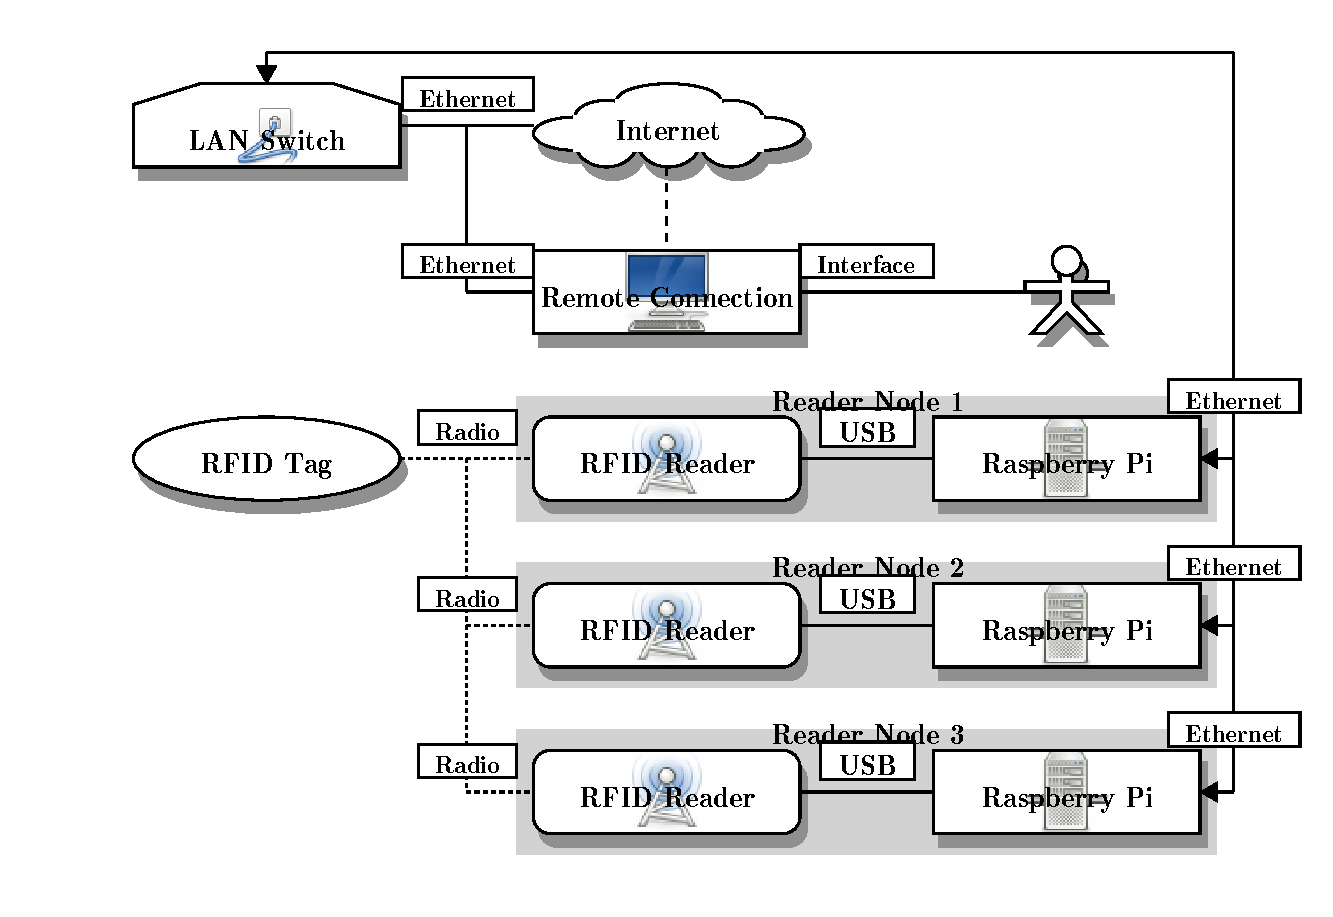
\includegraphics[width=1\textwidth]{figures/blockdiag/hardwaredesign}
		\caption{Hardware.}
		\label{fig:harddes}
	\end{center}
\end{figure}

\begin{figure}
	\begin{center}
		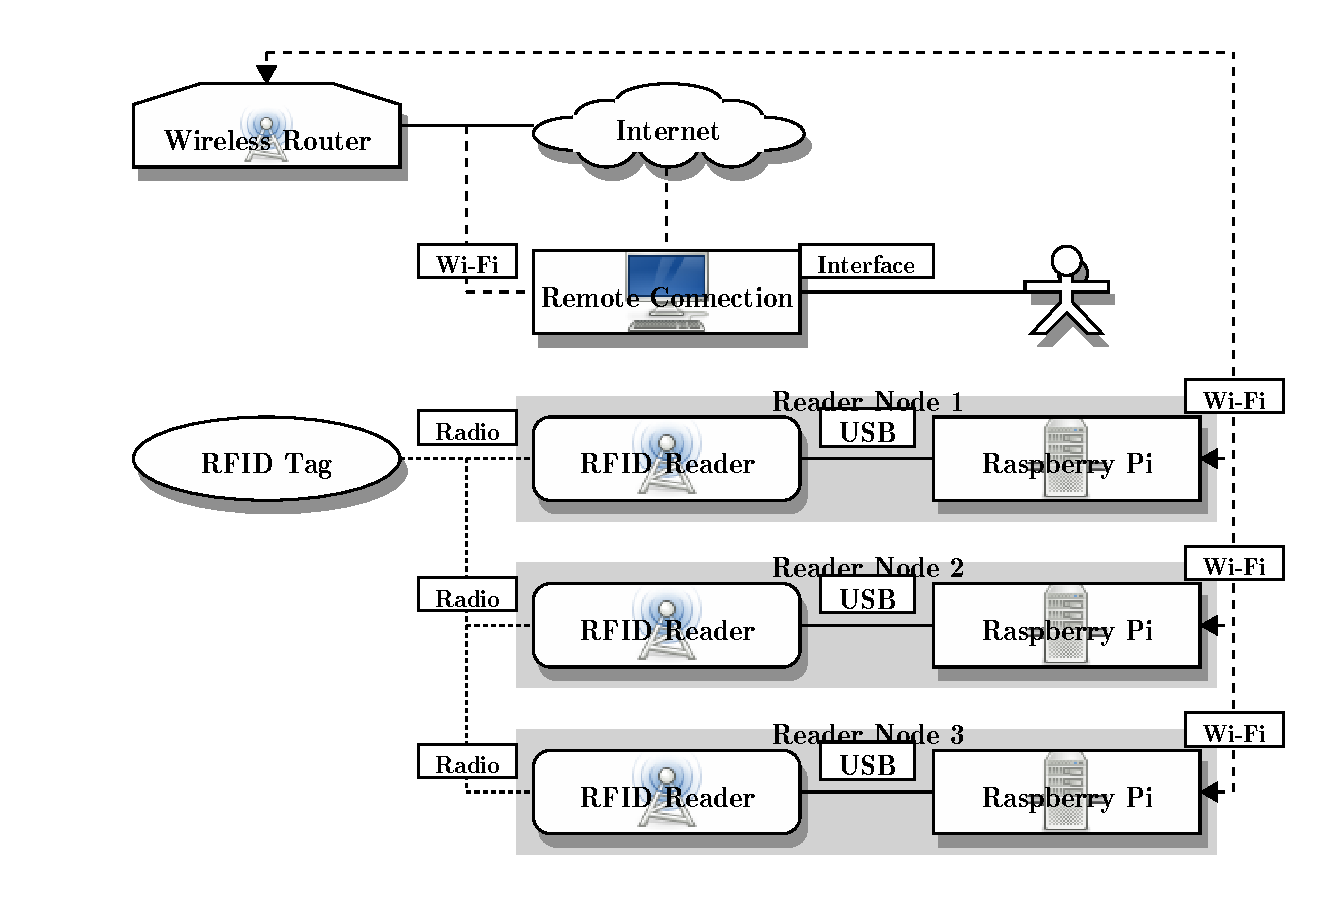
\includegraphics[width=1\textwidth]{figures/blockdiag/hardwaredesignwifi}
		\caption{Hardware Wifi.}
		\label{fig:harddeswifi}
	\end{center}
\end{figure}

\subsection{Antenna Design}

\section{Software design}
\label{sec:softdes}


\section{Summary}

\chapter{Implementation}
\label{ch:implementation}

This chapter describes how the system was built. Sections \ref{sec:projman} and \ref{sec:softengprac} present the software engineering tools and practices employed to aid the development process. Section \ref{sec:hardiss} explains the hardware problems that were encountered and how these were dealt with. Next, section \ref{sec:constread} goes through the steps taken to construct each reader node. Section \ref{sec:dataman} is concerned with how data was stored and managed in this system. Then, section \ref{sec:netcomm} describes how the reader nodes communicated RFID measurements over the network. Section \ref{sec:locest} explains how the methods for converting RSSI to distance and estimating the tag's location were implemented. Finally, section \ref{sec:webint} presents the web interface that was used to visualise the outputs of the system.

\section{Project management}
\label{sec:projman}

A number of considerations were taken into account when deciding how to manage this project. First, the system operates using a server-client model. This means that different software components are executing on multiple processing nodes. As a result, changes in one node need to be propagated in the whole system ensuring the consistency of the software.  Second, the software implementation is making use of different programming languages, multiple programming libraries, and a database management system. In order to ensure an iterative development process, where software components are constructed, debugged, and packaged together, it was decided to use the \textsc{Git} version control system\footnote{\textsc{Git} version control system - \url{http://git-scm.com/}}. This system keeps a distributed repository of all software and database files so that each node stores a copy of not only the whole software system, but also a complete history of changes. In addition, the use of a version control system stimulates the developer to merge a number of important changes into versions of the software. In this way, it becomes easy to track and monitor the project progress. The source code and documentation were hosted in a private repository on \textsc{GitHub}\footnote{The private project repository - \url{https://github.com/sandio/raspi-rfid-tracking}} with access granted to the people involved in developing and supervising the project.


\section{Software Engineering Practices}
\label{sec:softengprac}

A number of software engineering practices were of significant help when developing the RFID location sensing system. This section presents them and explains the problems that they solve.  

\subsection{Project decomposition}

It would have been a serious challenge to approach the project's task directly. The system consists of pieces of hardware that had to be orchestrated to solve a common problem. Therefore, it was very important to identify the system's components from early on. Hierarchical relationships between these parts were also defined. These steps ensured that the project could be divided into stages in order to systematically solve the main task. Regular deliveries of working components provided a more manageable way of constructing the final solution. For example, the work plan, devised before the start of the project, consisted of the following key activities:

\begin{enumerate}
 	\item Prepare the single-board computers
 	\item Construct functional RFID reader nodes
 	\item Receive information from the active RFID tag
 	\item Establish a network communication between nodes
 	\item Develop the localisation algorithm
 \end{enumerate}

Iterative construction of the system aided the development process. Problems and challenges were appearing gradually which helped solving them one at a time. 

\subsection{Object-oriented design}

This location sensing system is a combination of different software technologies. For instance, the system required an interface between a single-board computer and an RFID receiver. It also required means of communication between processing nodes. Logically, these and other requirements could be grouped into sets of functions, which is a motivation for employing an object-oriented design. This software methodology was used from the beginning of the project. Similar functionality is organised in a class. A class is responsible for all procedures concerning a particular part of the system. As a result, software is split into categories of functions, which makes it easy to address the class in charge of certain functionality.

Another benefit of the object-oriented design is modularity. For example, once input data is collected from all nodes it could be processed by a localisation algorithm in order to estimate the tag's position. Trilateration was chosen as the technique for computing locations. Object-oriented software development provides an easy way to experiment with different algorithms by substituting one class with another.

\subsection{System scalability}
\label{subsec:sysscal}

In this project, three single-board computers collaborate by exchanging RFID readings to localise a tagged object. Three reference points are needed in order to use trilateration in two dimensions  \cite{Zhang2009}. Nevertheless, more reader nodes could be used, in case multileration is implemented, to give a better approximation of a tag's position. Another scenario involves nodes disconnecting and later reappearing into the network. These possible cases show the dynamic nature of the system. It could scale up as the system grows, but also scale down if a reader node is faulty. This is an important property of the system, which was noted at the start of the project. To ensure scalability of the server-client model, the multi-threading programming model was used. It allows multiple threads to exist within the context of a single process. As a result, the system could concurrently receive RFID measurements from multiple reader nodes, update data structures, and compute the location of the unknown object.

\subsection{Documentation}

Writing documentation was an important part of this project. The source code of the system has been systematically documented throughout the development process. Using the inline comments specifying how the software components work, an Application Programming Interface (API) was constructed using \textsc{Sphinx}\footnote{\textsc{Sphinx} - a Python documentation generator - \url{http://sphinx-doc.org/index.html}}, a \textsc{Python} documentation generator. The API contains specifications of data structures, variables, and functions. It is a valuable source of information that provides a quick reference of how the system's components work and interact with each other. In addition, a manual for future users of the system was written. It gives a quick introduction of how to set up and use the system. The API and user manual can be viewed in Appendix \textbf{REF}  \textbf{TODO}.

This project consists of both hardware and software components. In order to clearly understand how hardware components are connected and how software objects interact, a number of diagrams were used in Chapter \textbf{REF} and in the user manual. These diagrams were generated using \textsc{Blockdiag} \footnote{\textsc{Blockdiag} - simple diagram images generator - \url{http://blockdiag.com/en/}} , a diagram image generator written in \textsc{Python}.

\section{Hardware Issues}
\label{sec:hardiss}

This section describes two hardware problems that were identified while the project was running. It also explains how these were solved.

\subsection{Antenna Design}
\label{subsec:antdes}

When the hardware equipment for this project arrived, everything was in order except for the RFID tag. It was missing its antenna, which is a coiled wire. The antenna needed to have specific length ($2cm$) and width ($8mm$) of the coil. The tag was being detected by the RFID readers but only in close range. Consequently, an antenna was required for the project to continue. A number of antennas were designed and soldered to the tag. Unfortunately, these were preventing the tag from being detected by the readers because they did not conform to the exact antenna specifications. The system could only receive measurements when these antennas were being touched by a human acting as an antenna extension. Another possible explanation was that the wires were composed of a bundle of smaller wire strings, which might have introduced interference in the radio transmission.

After a number of unsuccessful designs, an antenna was carefully constructed following the specifications of the manufacturer. Its wire was single and thick to ensure a strong signal would be emitted. Fortunately, this antenna worked perfectly and even increased the transmission range of the tag from eight meters as advertised by the manufacturer to 13 meters as identified during the hardware evaluation. The final antenna design can be seen on Figure \ref{fig:tag}.

\subsection{Serial to USB converters}
\label{subsec:sertousb}

The RFID readers communicate their measurements using a RS-232 serial port. The authors of the SpotON localisation system have identified the limitations of such serial connections \cite[p. 6]{Hightower2000}. This type of cabling is not universal and has limited length. Moreover, RS-232 serial ports are neither present on the Raspberry Pi computers, nor on most modern computers. In order to provide a convenient way of communication between an RFID reader and a Raspberry Pi, serial to USB converters were ordered along with the readers.

During the initial serial communication experiments, a problem was detected. When a serial connection is established, a flood of old identification and RSSI data filled the software input buffer of each Raspberry Pi. After in depth research of the issue, there was a strong indication that this could be caused by the chip of the serial to USB converters. This chip was sending data with high speeds, although the tag transmits its identity every two and a half to three seconds. 

This unexpected behaviour needed further investigation. One of the converters was taken apart, as seen on Figure \ref{fig:converter}. On the one hand, the sign on its case was indicating that it is model U-232-P9 manufactured by MCT Corp.. On the other hand, the chip model was PL2303HX detected by the Linux kernel as PL2303 manufactured by Prolific Technology, Inc.. Logically, one might ask what the brand of the converters was. In Linux, there is driver support for U-232-P9 as well. Attempts to use this driver instead of the automatically detected one resulted in a system crash. Further research indicated that this chip (PL2303HX) is an imitation of a genuine Prolific Technology chip \footnote{Prolific Technology Inc. PL2303 Windows Driver Download - \url{http://www.prolific.com.tw/US/ShowProduct.aspx?p_id=225&pcid=41}}. At this point, it was known that these converters were cheaper counterfeits. Nevertheless, they did work but flooded the computers' input buffers at the start of every serial connection.

\begin{figure}[h]
	\begin{center}
		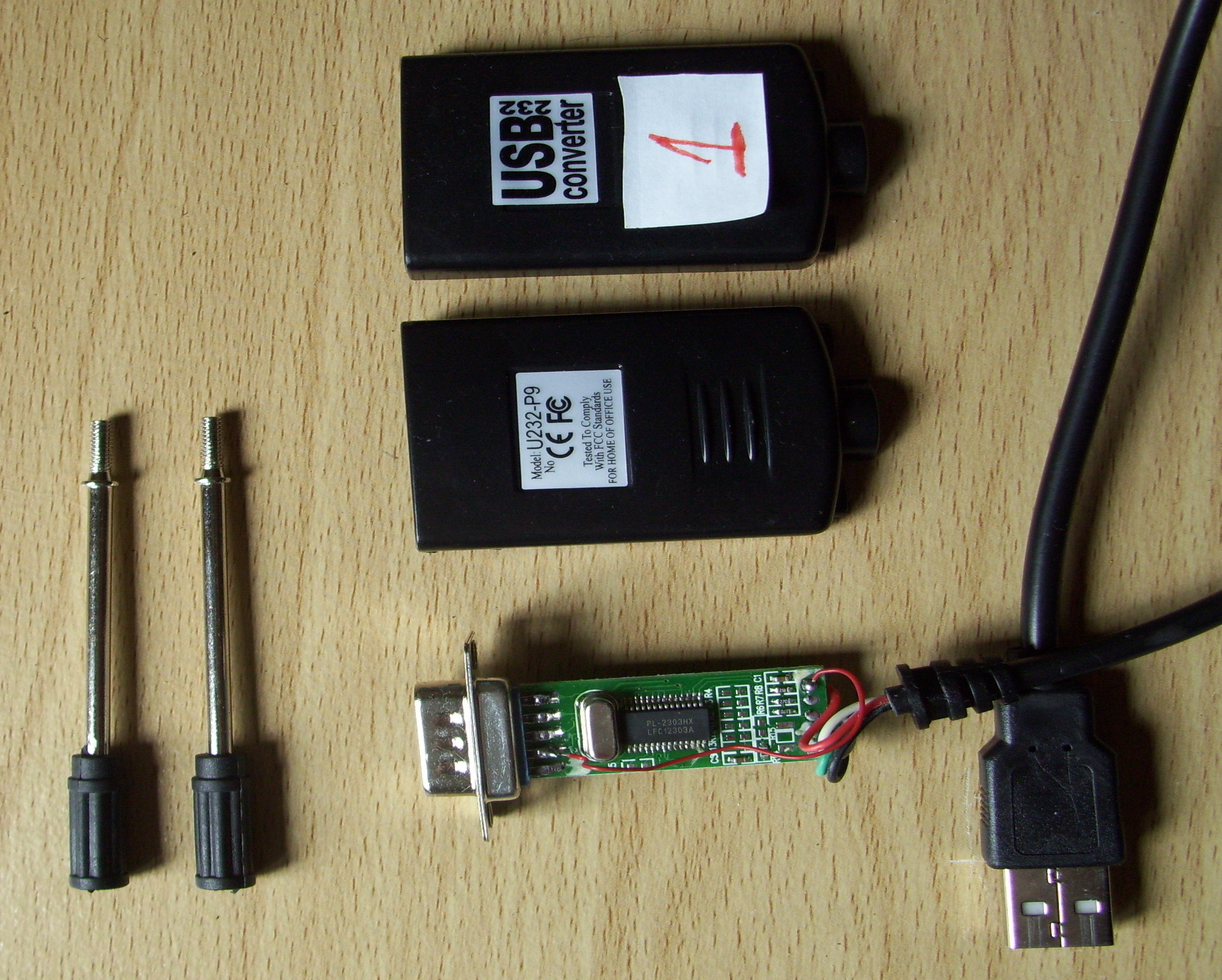
\includegraphics[width=.6\textwidth]{figures/converter2}
		\caption{The disassembled serial to USB converter.}
		\label{fig:converter}
	\end{center}
\end{figure}

The solution that worked best is to repeatedly drain the operating system input buffer until it holds a few bytes, an indication that the devices are communicating normally. A drawback of this approach is the time lost until the communication stabilises. Up to 58 initial buffer drains were recorded. A third of a second was chosen as a waiting time between buffer drains to ensure the operating system had time to perform this operation. This resulted in a maximum of 17.4 seconds ($58 \times 0.3s$) initial waiting time before the system could starts its normal operation. In addition, each of the nodes had to not only wait between zero and a maximum time, but also ensure the other nodes had drained their buffers. This is because readings from all three nodes were needed for estimating the position of the tag. Due to the hardware nature of the problem, time would always be lost until different converters are tested.


\section{Reader nodes construction}
\label{sec:constread}

Constructing the reader nodes consisted of three main steps. First, an operating system had to be installed on each of the Raspberry Pi computers. The Raspbian Linux distribution\footnote{Raspbian Linux website - \url{http://www.raspbian.org/}} was selected because it is specifically optimised for these single-board computers and has a rich software base compiled for the ARM processor architecture. Second, the RFID readers and Raspberry Pi computers were connected through USB. Third, a software interface between the devices was implemented.

Most of the system was programmed in the \textsc{Python} programming language. All functions concerned with the serial communication of the devices were grouped together in a class called \textsf{SerialConnection}. The \textsc{pyserial} module was extensively used to implement the required functionality. The class consisted of methods for initialising a serial connection on a given port (\verb!/dev/ttyUSB0!), opening and closing this port for communication, flushing the input buffer, and reading incoming data. The last function had to be implemented to parse the information arriving from the readers. Most serial devices separate their individual readings by a newline character (\verb!\n!), carriage return (\verb!\r!), or a combination of the both (\verb!\n\r!). These readers, however, separate measurements by a space character. As a result, \textsc{pyserial} functions for reading data could not be used. The solution implemented reads incoming information character by character until the separator is encountered. All methods provided by the \textsf{SerialConnection} class are illustrated as a sequence diagram on Figure \ref{fig:seqserial}.

\begin{figure}[h]
	\begin{center}
		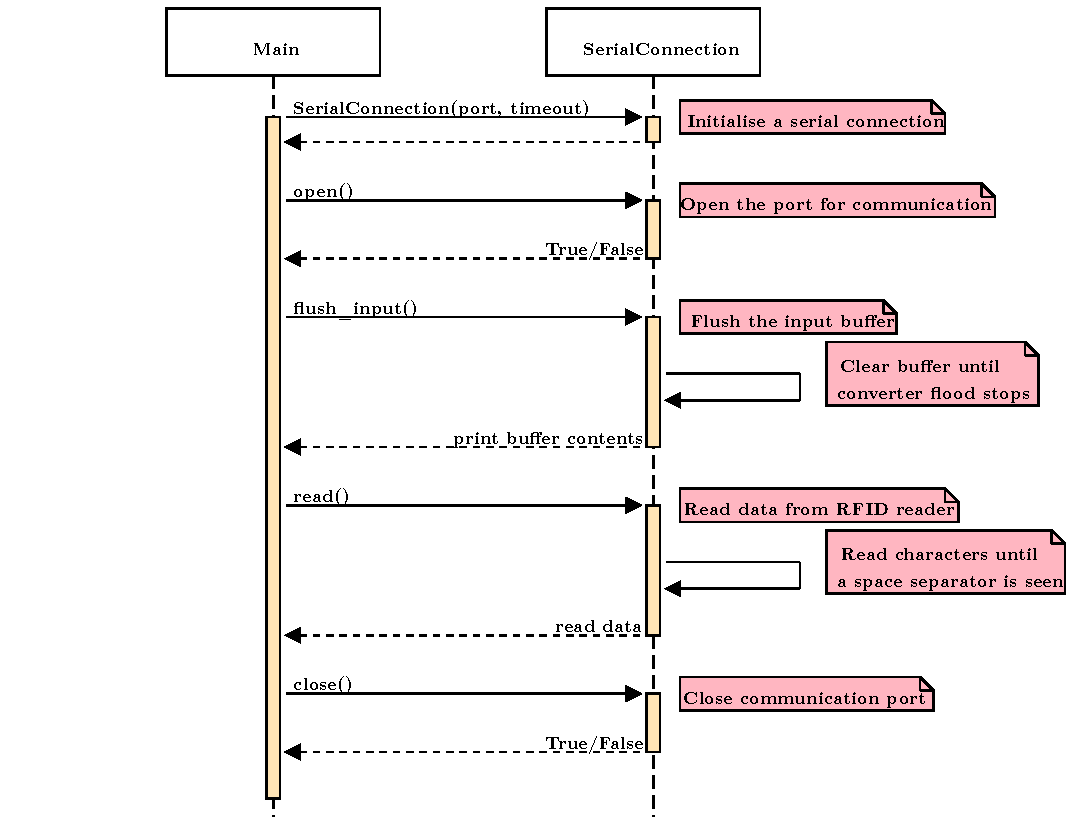
\includegraphics[width=1\textwidth]{figures/seqdiag/serial}
		\caption{A sequence diagram illustrating the methods of the \textsf{SerialConnection} class. The usual sequence in which they are called is shown from top to bottom.}
		\label{fig:seqserial}
	\end{center}
\end{figure}

\section{Data store and management}
\label{sec:dataman}

In this project, there were a number of important data fields that need to be accessed by processes and threads. For example, as discussed in section \ref{subsec:sysscal}, the system employed a server-client model where the server consisted of threads that simultaneously receive RFID readings from the other two nodes. These measurements needed to be stored but also retrieved by the localisation algorithm or by the website visualiser, presented in section \ref{sec:webint}. This was a motivation for employing a data structure that was independent of the software components of the system. Support for simultaneous access of the data was also required.

The \textsc{SQLite}\footnote{\textsc{SQLite} website - \url{http://www.sqlite.org/}} database management system met the above requirements. It is a file-based system that operates without a server process, which spares system resources. \textsc{SQLite} serialises transactions so that all changes appear atomic and do not overlap in time. Database transactions might happen in parallel but are processed in a sequential order by the database management system. Queries to the database were implemented in functions part of the \textsf{DatabaseHandler} class. Instances of this class were created in other classes where access to data was required.

Important data fields were the RFID readings, the positions of the reader nodes, and the estimated location of the RFID tag. These were stored in database tables. Examples of such data are shown in Table \ref{tbl:sample}.

\begin{table}[h]
	\centering
	\begin{subtable}[b]{1\textwidth}
	\centering
	\begin{tabular}{|c|c|c|c|}
		\hline
		Reading & Node N\textsuperscript{\underline{o}} & Tag Id 	& RSSI	\\ \hline
		1		& 0										& 1Fwt		& 44	\\ \hline
		2		& 2										& 1Fwt		& 78	\\ \hline
		3		& 1										& 1Fwt		& 48	\\ \hline
		4		& 0										& 1Fwt		& 43	\\ \hline
	\end{tabular}
	\caption{Top four reader measurements.}
	\end{subtable}
	
	\begin{subtable}[b]{1\textwidth}
	\centering
	\begin{tabular}{|l|c|c|c|c|c|}
		\hline
		Node	& Node N\textsuperscript{\underline{o}} & $x$ 	& $y$ & $z$ & radius	\\ \hline
		Reader	& 0 									& 0.0 	& 3.0 & 0.0 & 4.0		\\ \hline
		Reader	& 1 									& 3.0 	& 0.0 & 0.0 & 0.786		\\ \hline
		Reader	& 2 									& 0.0 	& 0.0 & 0.0 & 5.0		\\ \hline
		Tag		& 3 									& 5.563 & 3.0 & 0.0 & 0.0		\\ \hline
	\end{tabular}
	\caption{Object positions in two dimensions.}
	\end{subtable}
	
	\caption{Sample data from the database of the system.}
	\label{tbl:sample}
\end{table}


\section{Network communication}
\label{sec:netcomm}

The overall software design of the system was introduced in section \ref{sec:softarch}. It defined the server-client model used to communicate RFID readings over a computer network. This section is concerned with detailing how this network communication was implemented.

Two of the Raspberry Pi computers acted as nodes that gathered information from their RFID readers to immediately send it over the network to the third node. This node was designated as the server of the system collecting readings and using this information to compute the tag's position. The network communication was implemented using socket programming. Python's \textsc{socket} module offered all required functions.

At the client side, the \textsf{NetworkClient} class was responsible for initialising a client streaming socket. A client  can only use a client socket to connect to a server socket. A streaming socket was chosen because nodes communicate a continuous stream of data to the server node. After this socket is created, a connection request is sent to a server socket specifying the network address and port of the server computer.

At the server side, the \textsf{NetworkServer} class creates a server streaming socket. Next, this socket is bound to the network address of the machine on a specified port. Then, the server socket starts listening for incoming connections. The server checks for connection requests using a non-blocking approach. This means that the programme tests if a request is available without indefinitely waiting for one to arrive, thus being able to terminate if requested. Once a client tries to connect, the \textsf{NetworkServer} accepts it by creating a client socket at the server side. At this point the only thing left to serve the incoming request is for the server to spawn a thread that handles the connection from this moment on. The motivation for using a threaded network server is discussed in section \ref{subsec:sysscal}.

Each network server thread receives incoming data from one client node. Listening on the socket for new information is again implemented using a non-blocking socket. If the receive buffer is empty, the receiver thread will not block indefinitely until data arrives. Rather this buffer is checked constantly but the thread could still be controlled by its parent process. If new data is available, it is read and inserted into the database using an instance of the \textsf{DatabaseHandler} class.

In case the system is interrupted by the user, the network server sends a stop signal to each of its threads and waits for them to terminate individually before terminating itself. This is the behaviour of the \textsf{join(timeout)} function of the Python's \textsf{threading} module. All the functionality described above is illustrated as a sequence diagram on Figure
\ref{fig:seqnet}.

\begin{figure}[h]
	\begin{center}
		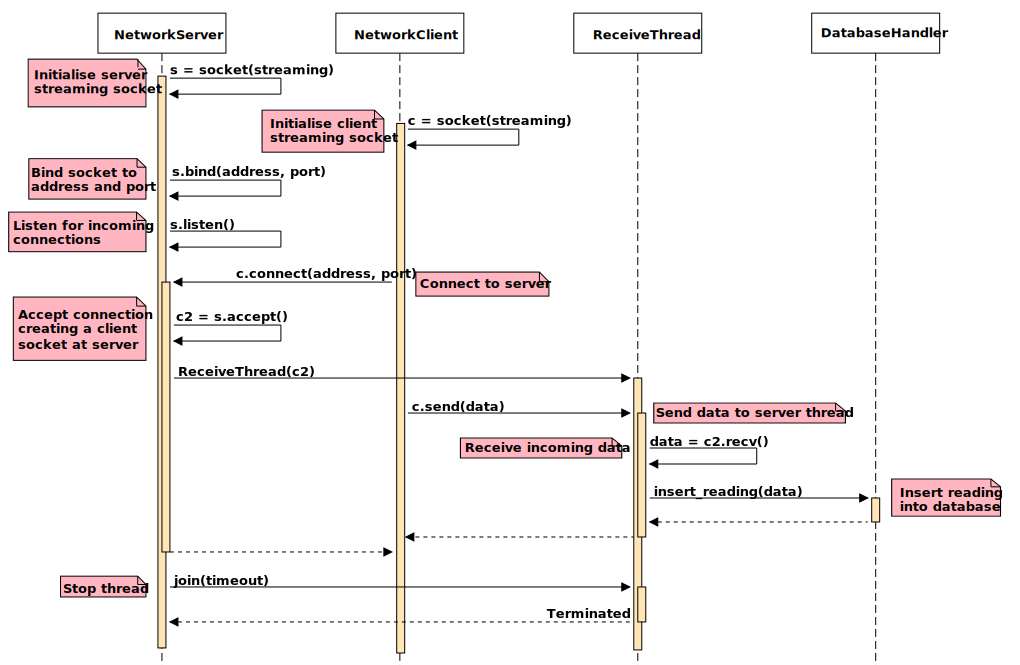
\includegraphics[width=1\textwidth]{figures/seqdiag/network}
		\caption{A sequence diagram illustrating the methods of the \textsf{NetworkServer}, \textsf{NetworkClient}, and \textsf{ReceiveThread} classes. The usual sequence in which they are called is shown from top to bottom.}
		\label{fig:seqnet}
	\end{center}
\end{figure}

\section{Location estimation}
\label{sec:locest}

This section presents the implementation details of converting RSSI to distance and computing the unknown position of the RFID tag using the trilateration technique.

\subsection{RSSI to distance conversion}

The implementation of converting RSSI to distance closely followed the methodology described in section \ref{subsec:transtbl}. More specifically, the programme uses an instance of the \textsf{DatabaseHandler} class to get the three most recent RFID readings from the database. For each of these, an RSSI value is converted to distance in meters based on the translation table of the reader at which the measurement was recorded. This is needed because of the slight hardware differences between the RFID readers. Next, an integer factor is added to an RSSI value to account for the battery power drop as it is being used. Then, the position of an RSSI measurement in the translation table is determined. Finally, RSSI is linearly converted to distance for the specific range.

\subsection{Trilateration}
\label{subsec:trilatimpl}


The trilateration position estimation technique was implemented relying on the general three-dimensional solution of the method presented in section \ref{sec:trilatmeth}. The algorithm accepts as inputs the positions of the three reader nodes and their RSSI measurements. The positions are fetched from the database and the RSSI values are converted to distance using the aforementioned steps. The all the equations of the trilateration method were directly implemented with the aid of the \textsc{math} (mathematical functions) and \textsc{numpy} (scientific computing) modules. It was noted that a number of recurring intermediate computations could be computed once and inserted in the equations as variables. Such computations included $\vec p_2 - \vec p_1$, $\vec p_3 - \vec p_1$, and $\hat e_x i$. The algorithm outputs the estimated location of the unknown object. This result is inserted into the database so that it could be visualised on the web interface.

\section{Web Interface}
\label{sec:webint}

The web interface is a website that runs on the server node. It main purpose is to provide a convenient interface to interact with the system. The web page is automatically refreshed every three seconds, which is roughly the interval at which the RFID tag transmits its identity. The website provides the following information:

\begin{itemize}
	\item the positions of the readers and tag,
	\item a form to change the positions of the reader nodes,
	\item the error in meters of the estimated position to the true one,
	\item a graph with reader positions and their distance from the tag,
	\item a table with the three most recent RFID readings,
	\item a table providing status information about the Raspberry Pis. 
\end{itemize}

The website is implemented in the \textsc{PHP} programming language. All information is provided from the \textsc{SQLite} database. The website runs on an \textsc{Apache} HTTP web server installed on the server node. The website was password protected to allow only people involved in this project to access it through the Internet. Figure \ref{fig:web} is screen capture of the web interface.

\begin{figure}[h]
	\begin{center}
		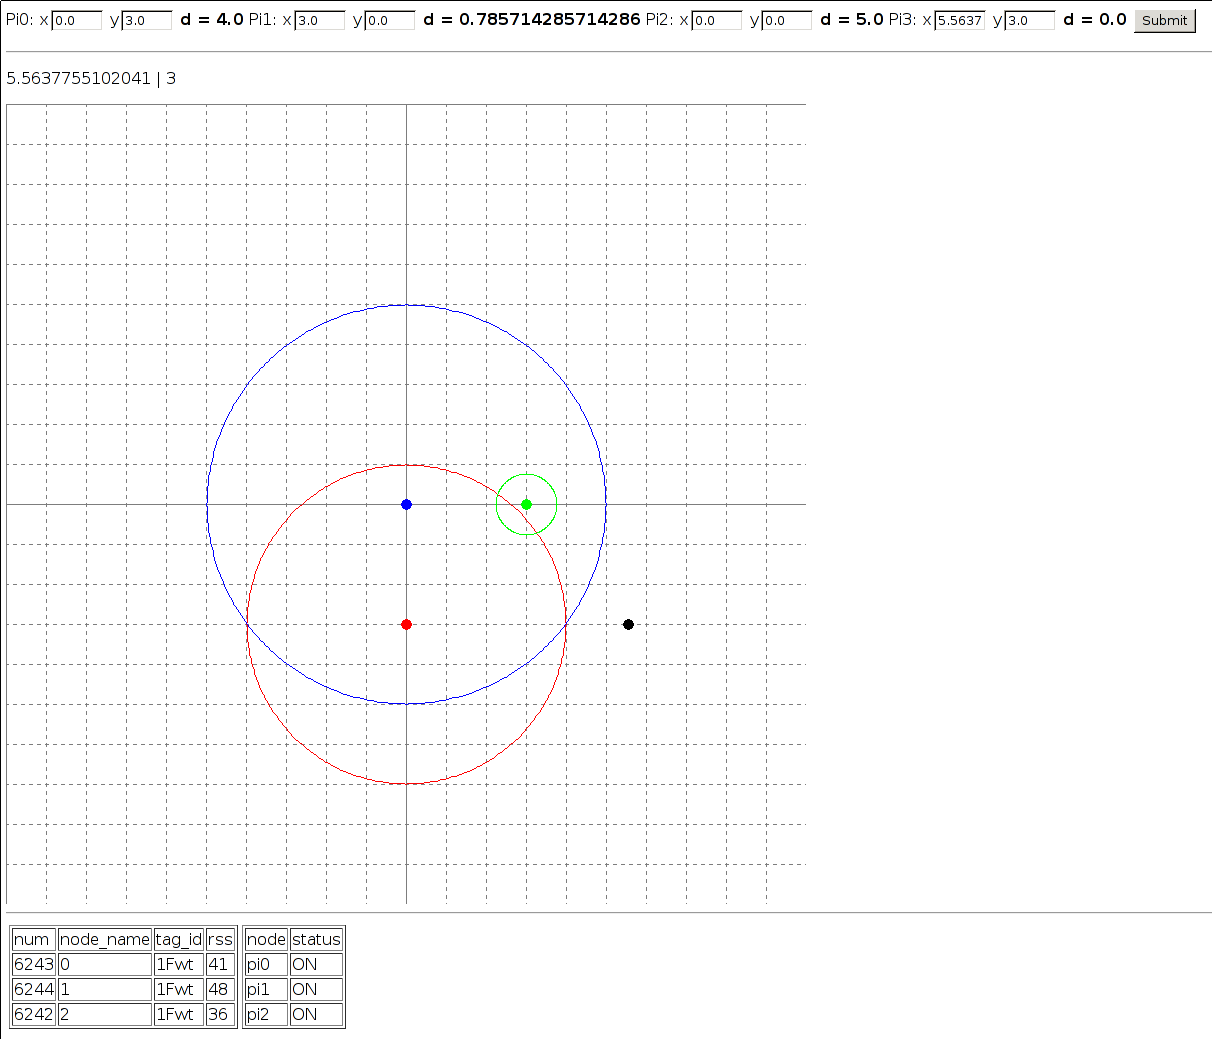
\includegraphics[width=.8\textwidth]{figures/sim}
		\caption{The web interface running on the server node.}
		\label{fig:web}
	\end{center}
\end{figure}


\section{Summary}

This chapter detailed the software practices that helped develop this system. It also described hardware issues that were faced throughout the project. Next, implementation details of all parts of the system were presented. The next chapter discusses the evaluation of the system's hardware component and the overall system's performance in terms of localisation accuracy.

\chapter{Evaluation}
\label{ch:evaluation}

\begin{figure}
	\begin{center}
		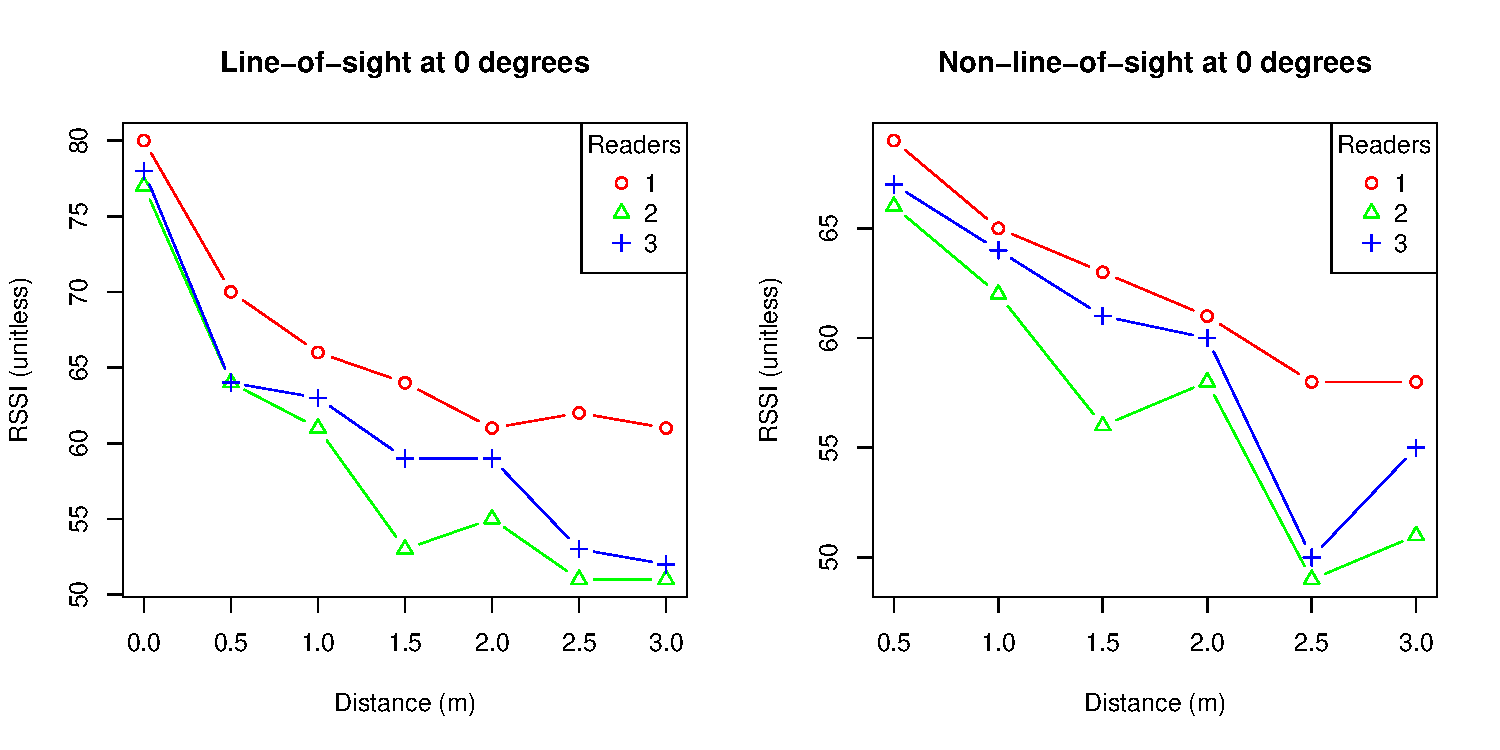
\includegraphics[width=1\textwidth]{figures/rssi_distance_3m_0deg}
		\caption{Two plots of RSSI measurements at increasing distances with the readers at 0 degrees (antennas facing the tag). The left graph show how RSSI values change with a line-of-sight signal propagation. The right graph illustrates the same experiment but with a non-line-of-sight signal propagation (there is an obstacle between the reader and the tag).}
	\end{center}
\end{figure}
\begin{figure}
	\begin{center}
		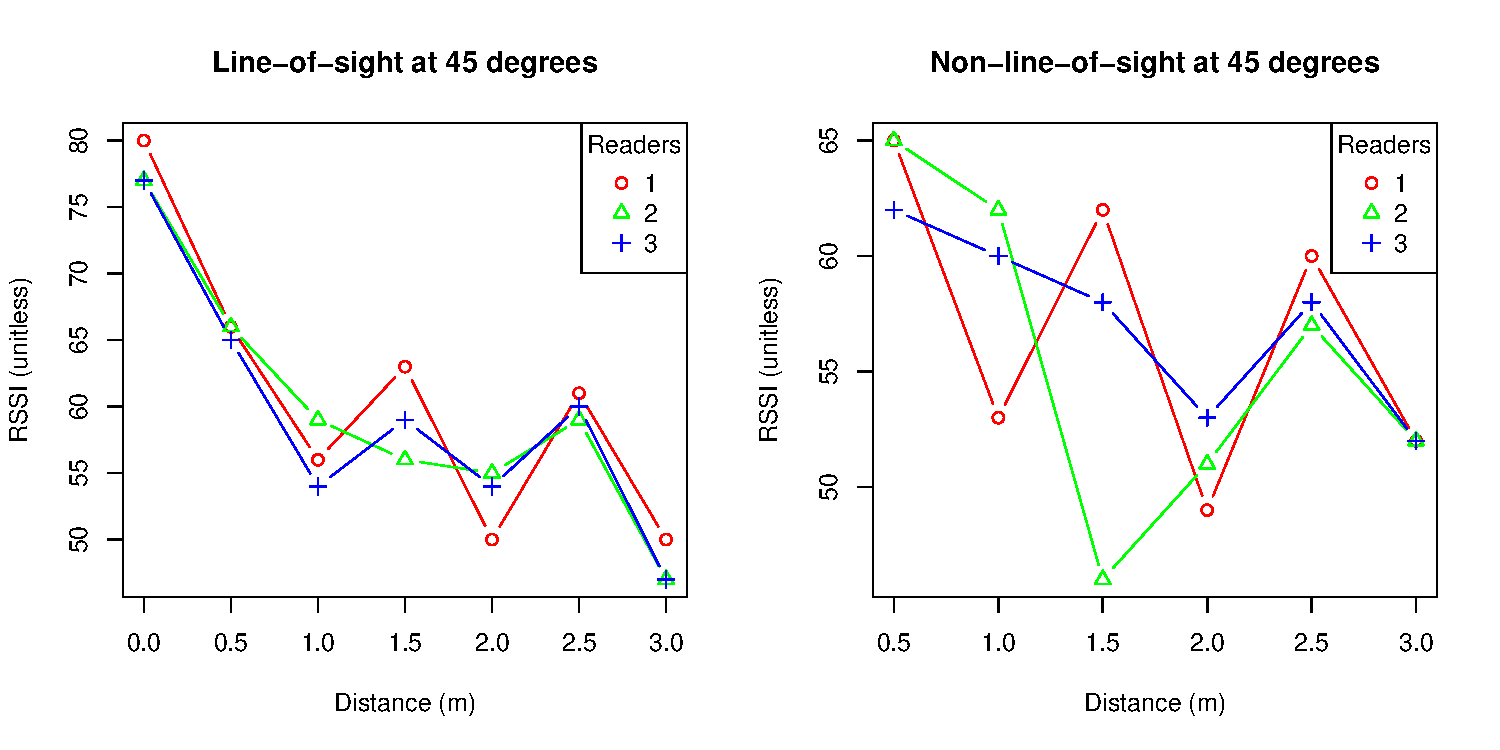
\includegraphics[width=1\textwidth]{figures/rssi_distance_3m_45deg}
		\caption{Two plots of RSSI measurements at increasing distances with the readers at 45 degrees (antennas at an angle to the tag). The left graph show how RSSI values change with a line-of-sight signal propagation. The right graph illustrates the same experiment but with a non-line-of-sight signal propagation (there is an obstacle between the reader and the tag).}
	\end{center}
\end{figure}
\begin{figure}
	\begin{center}
		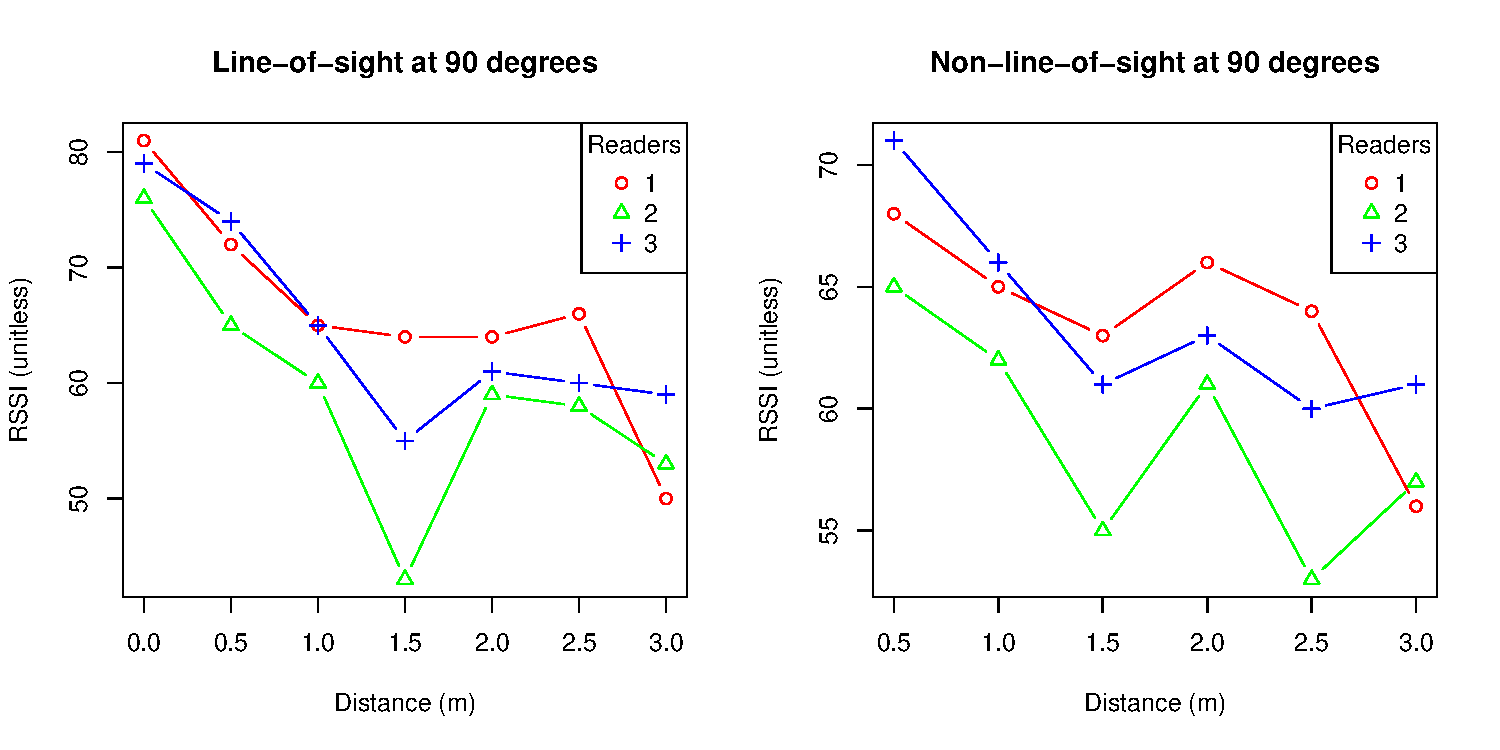
\includegraphics[width=1\textwidth]{figures/rssi_distance_3m_90deg}
		\caption{Two plots of RSSI measurements at increasing distances with the readers at 90 degrees (antennas at an angle to the tag). The left graph show how RSSI values change with a line-of-sight signal propagation. The right graph illustrates the same experiment but with a non-line-of-sight signal propagation (there is an obstacle between the reader and the tag).}
	\end{center}
\end{figure}
\begin{figure}
	\begin{center}
		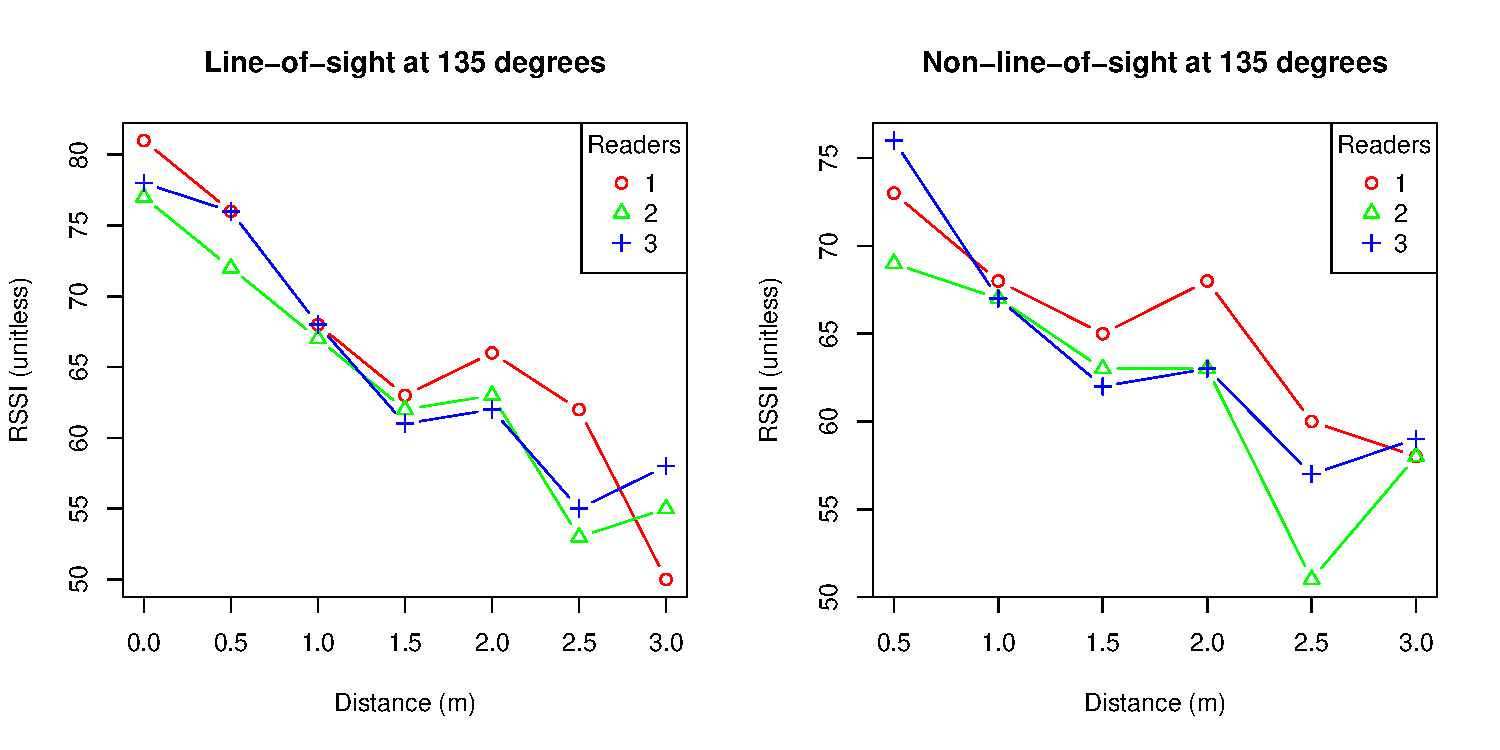
\includegraphics[width=1\textwidth]{figures/rssi_distance_3m_135deg}
		\caption{Two plots of RSSI measurements at increasing distances with the readers at 135 degrees (antennas at an angle to the tag). The left graph show how RSSI values change with a line-of-sight signal propagation. The right graph illustrates the same experiment but with a non-line-of-sight signal propagation (there is an obstacle between the reader and the tag).}
	\end{center}
\end{figure}
\begin{figure}
	\begin{center}
		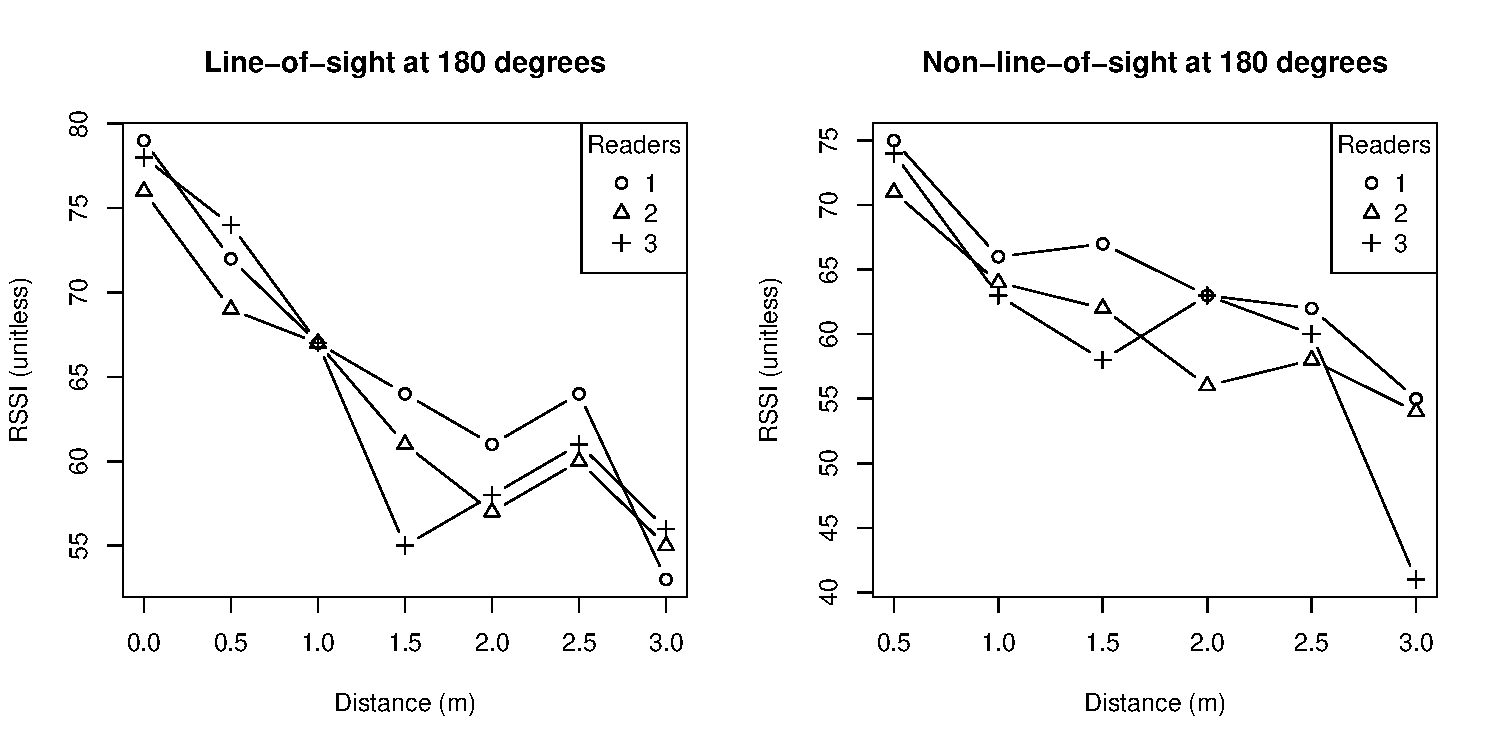
\includegraphics[width=1\textwidth]{figures/rssi_distance_3m_180deg}
		\caption{Two plots of RSSI measurements at increasing distances with the readers at 180 degrees (antennas at an angle to the tag). The left graph show how RSSI values change with a line-of-sight signal propagation. The right graph illustrates the same experiment but with a non-line-of-sight signal propagation (there is an obstacle between the reader and the tag).}
	\end{center}
\end{figure}
\begin{figure}
	\begin{center}
		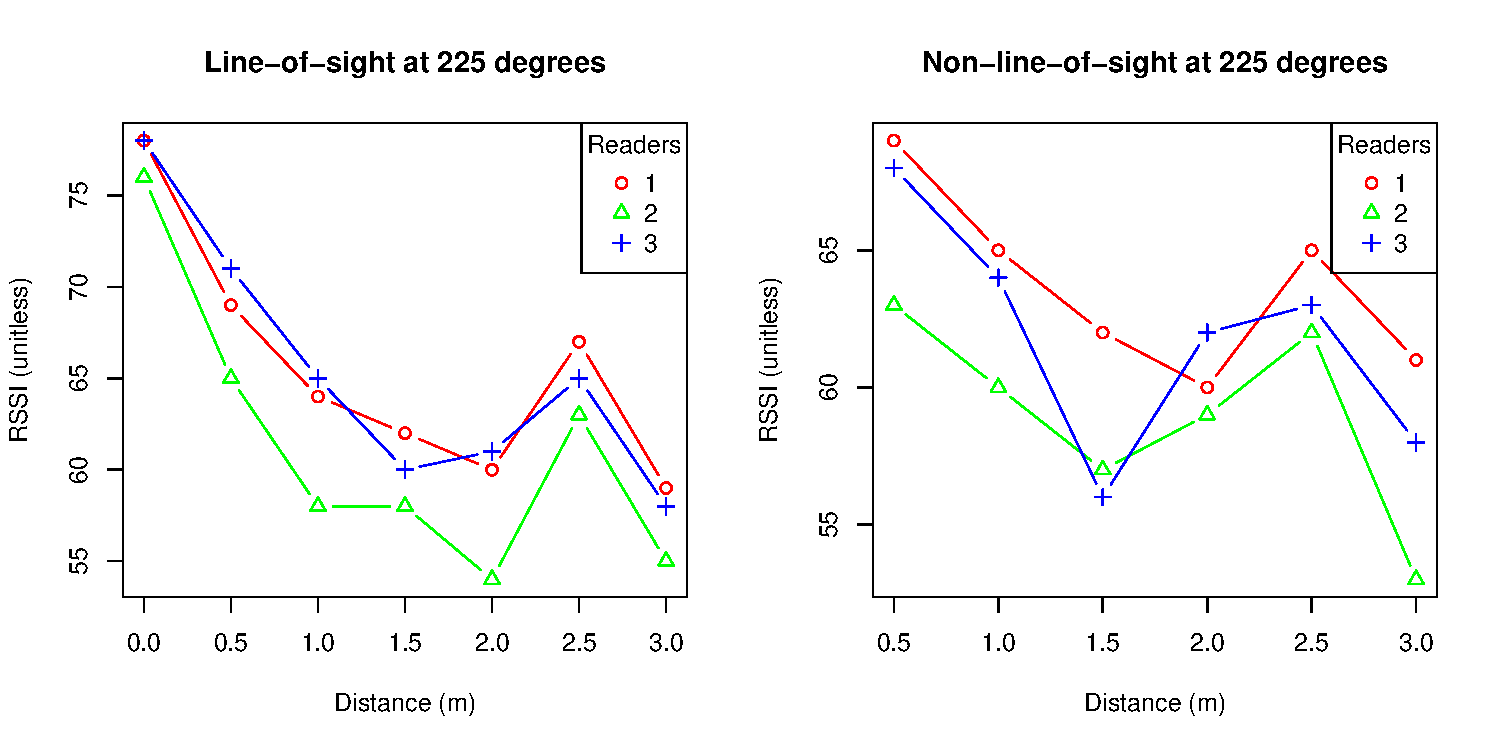
\includegraphics[width=1\textwidth]{figures/rssi_distance_3m_225deg}
		\caption{Two plots of RSSI measurements at increasing distances with the readers at 225 degrees (antennas at an angle to the tag). The left graph show how RSSI values change with a line-of-sight signal propagation. The right graph illustrates the same experiment but with a non-line-of-sight signal propagation (there is an obstacle between the reader and the tag).}
	\end{center}
\end{figure}
\begin{figure}
	\begin{center}
		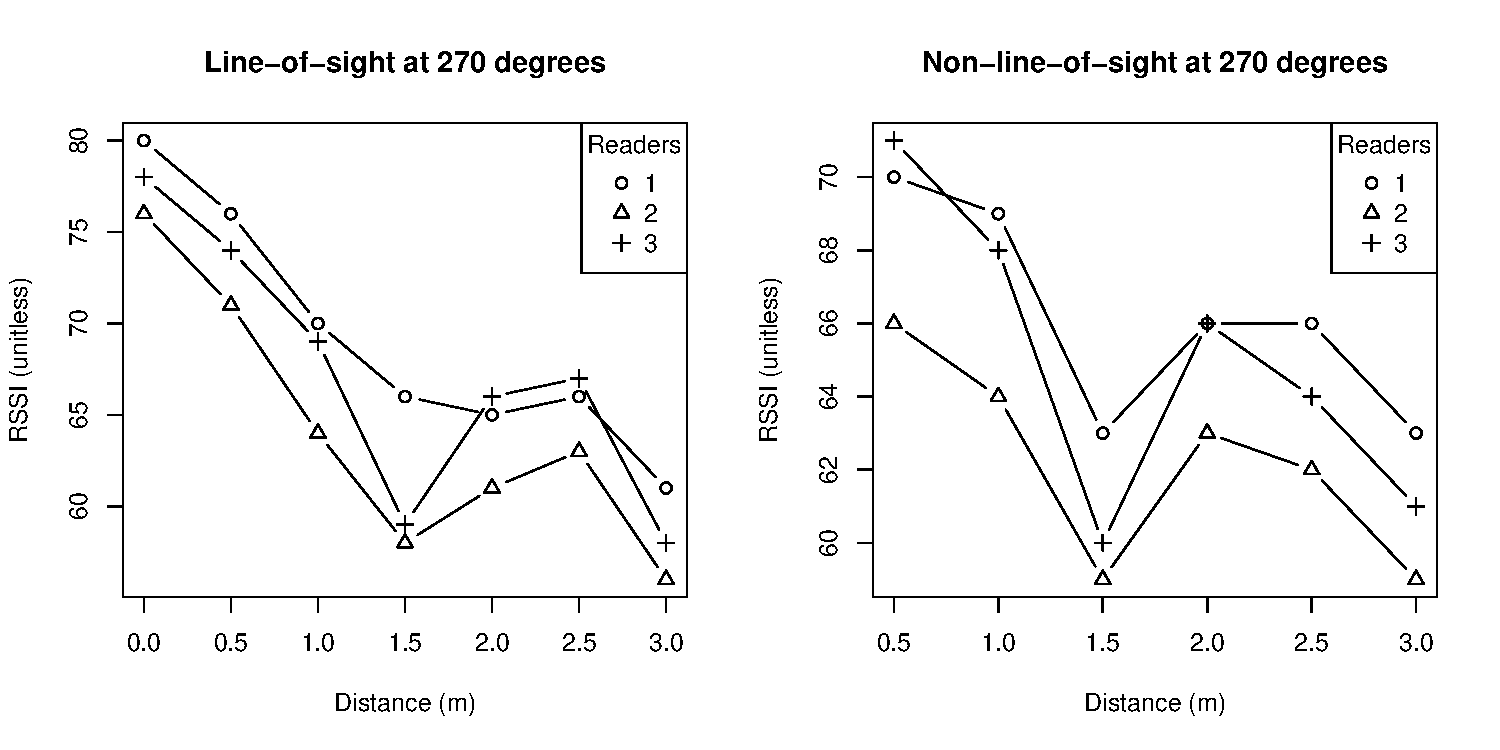
\includegraphics[width=1\textwidth]{figures/rssi_distance_3m_270deg}
		\caption{Two plots of RSSI measurements at increasing distances with the readers at 270 degrees (antennas at an angle to the tag). The left graph show how RSSI values change with a line-of-sight signal propagation. The right graph illustrates the same experiment but with a non-line-of-sight signal propagation (there is an obstacle between the reader and the tag).}
	\end{center}
\end{figure}
\begin{figure}
	\begin{center}
		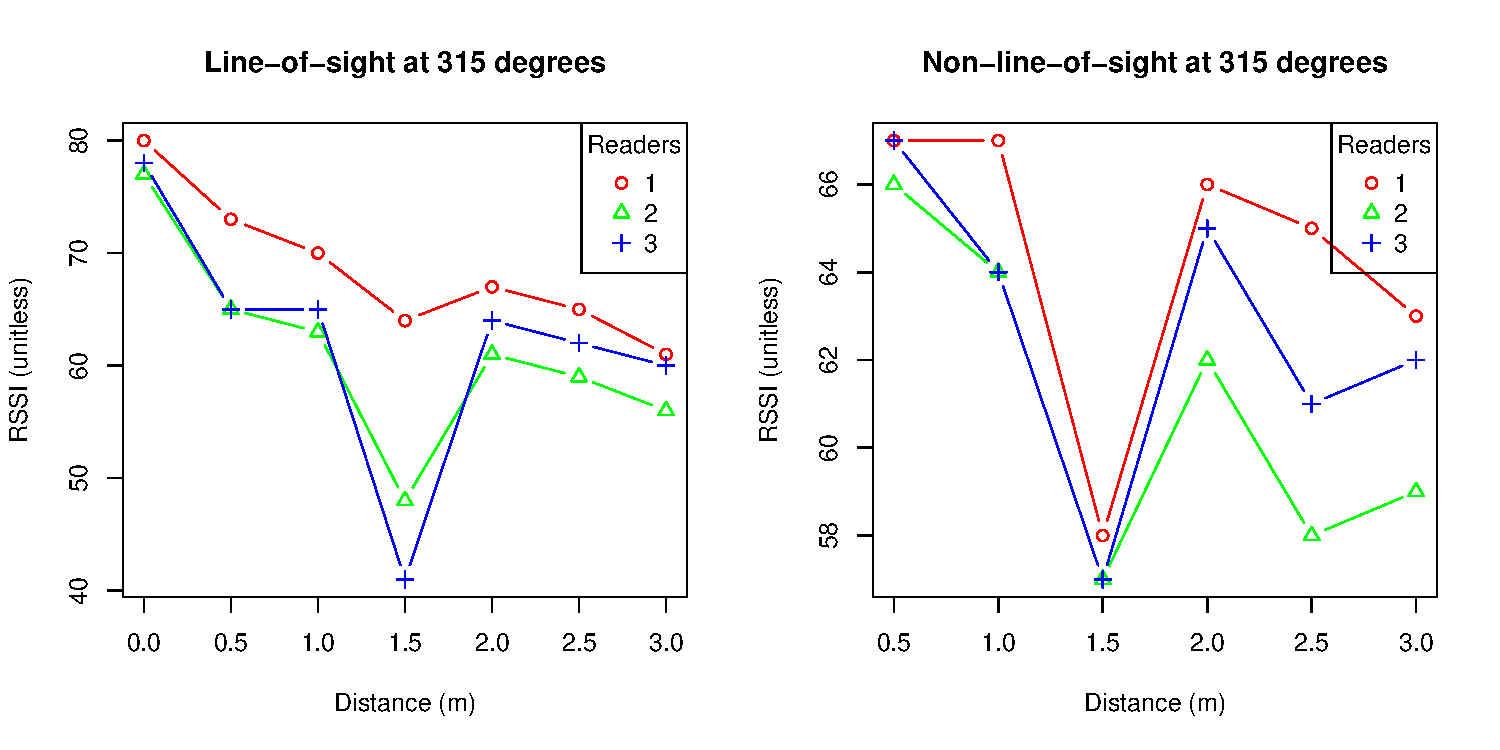
\includegraphics[width=1\textwidth]{figures/rssi_distance_3m_315deg}
		\caption{Two plots of RSSI measurements at increasing distances with the readers at 315 degrees (antennas at an angle to the tag). The left graph show how RSSI values change with a line-of-sight signal propagation. The right graph illustrates the same experiment but with a non-line-of-sight signal propagation (there is an obstacle between the reader and the tag).}
	\end{center}
\end{figure}
\begin{figure}
	\begin{center}
		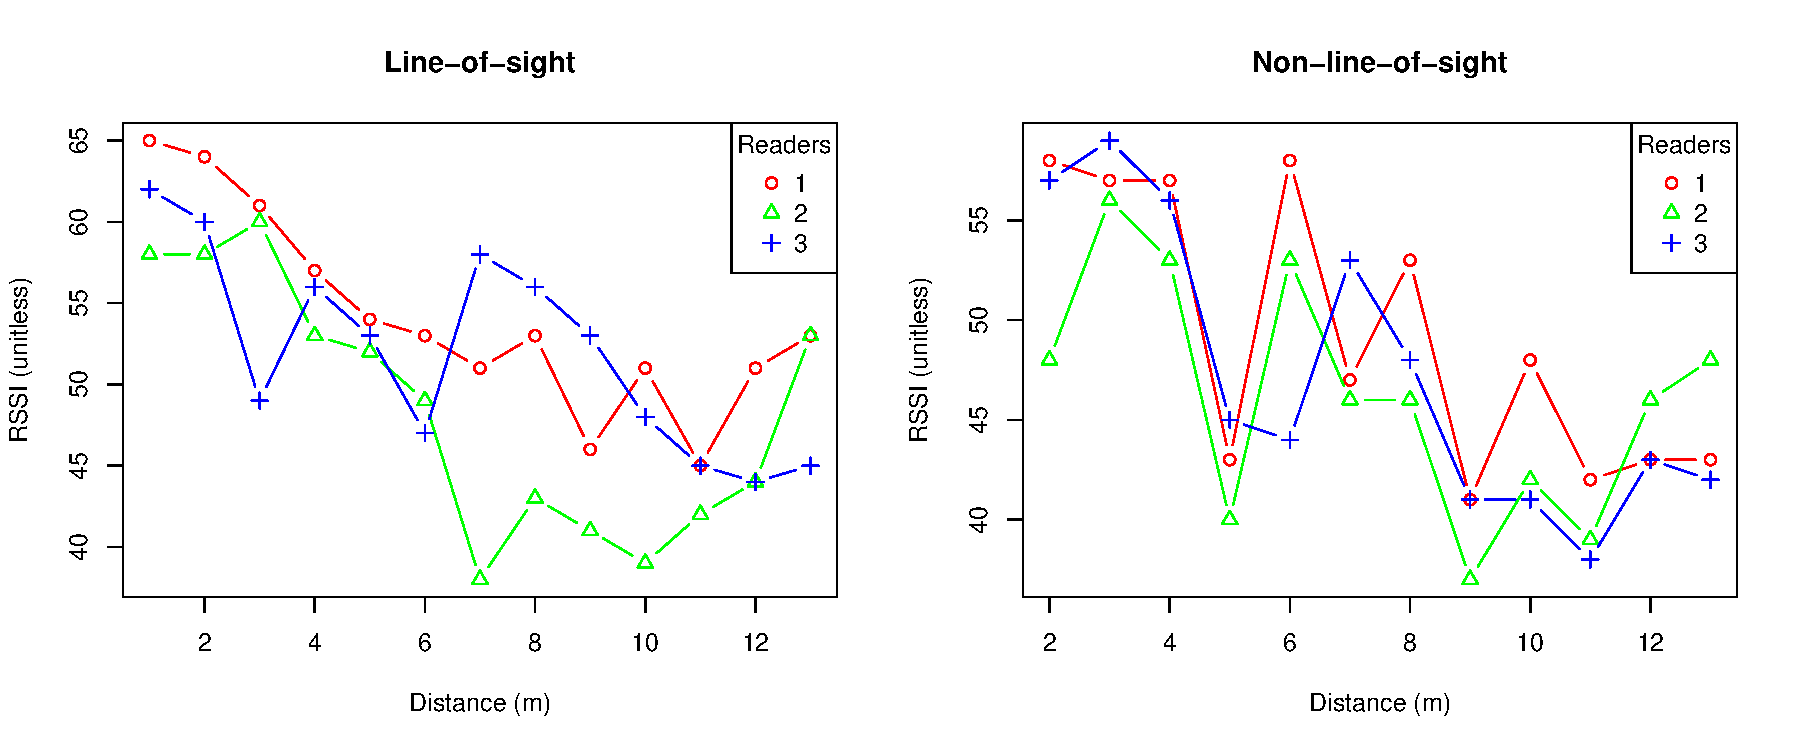
\includegraphics[width=1\textwidth]{figures/rssi_distance_13m}
		\caption{Two plots of RSSI measurements at increasing distances with the readers facing the tag. The left graph show how RSSI values change with a line-of-sight signal propagation. The right graph illustrates the same experiment but with a non-line-of-sight signal propagation (there is an obstacle between the reader and the tag).}
	\end{center}
\end{figure}
\begin{figure}
	\begin{center}
		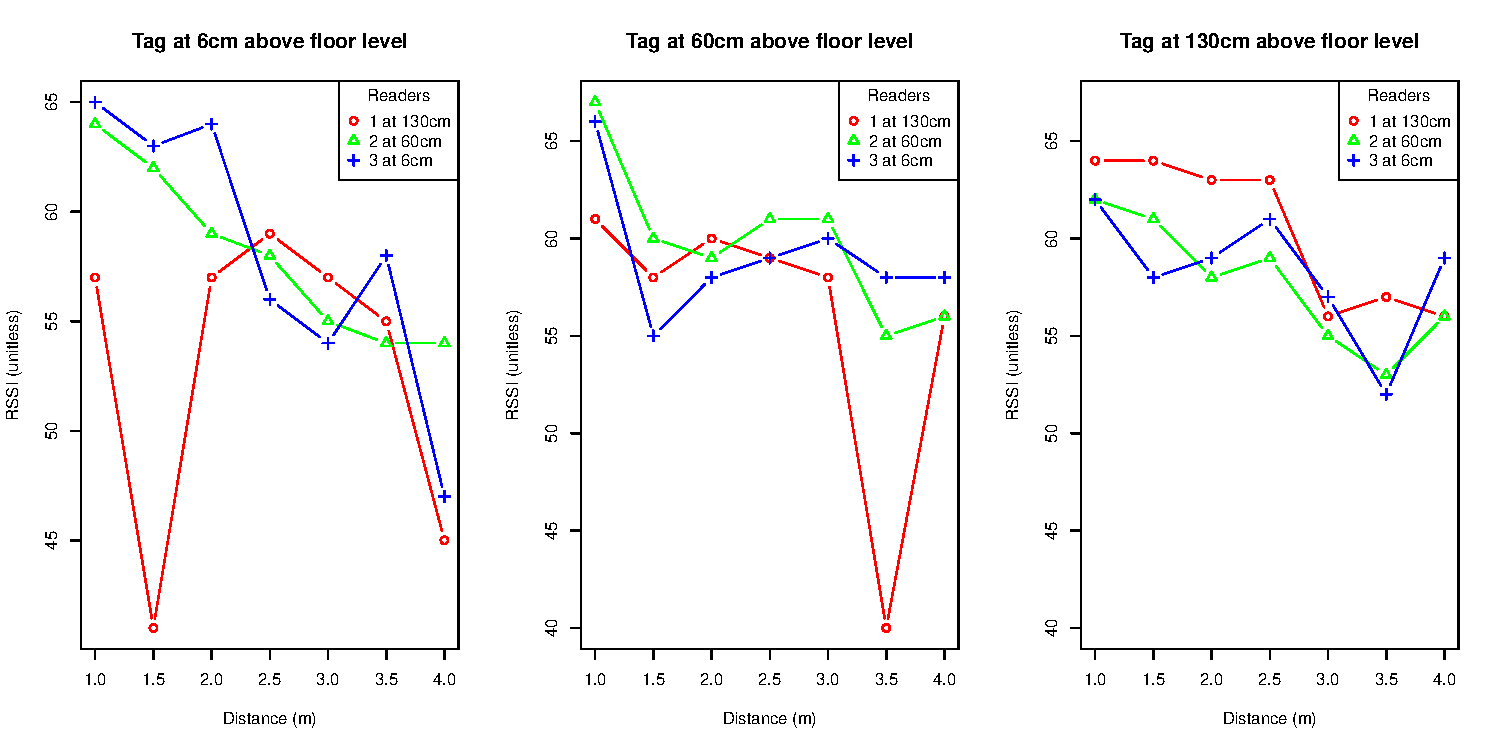
\includegraphics[width=1\textwidth]{figures/rssi_distance_4m}
		\caption{Three plots of RSSI measurements at increasing distances with the readers at different elevation from the floor in an indoor environment. The first graph shows how RSSI measurements change as the distance grows when the tag is placed at 6cm above floor level. The second and third graph show the same experiment but the tag is at 60cm and 130cm above the floor level.}
	\end{center}
\end{figure}
\begin{figure}
	\begin{center}
		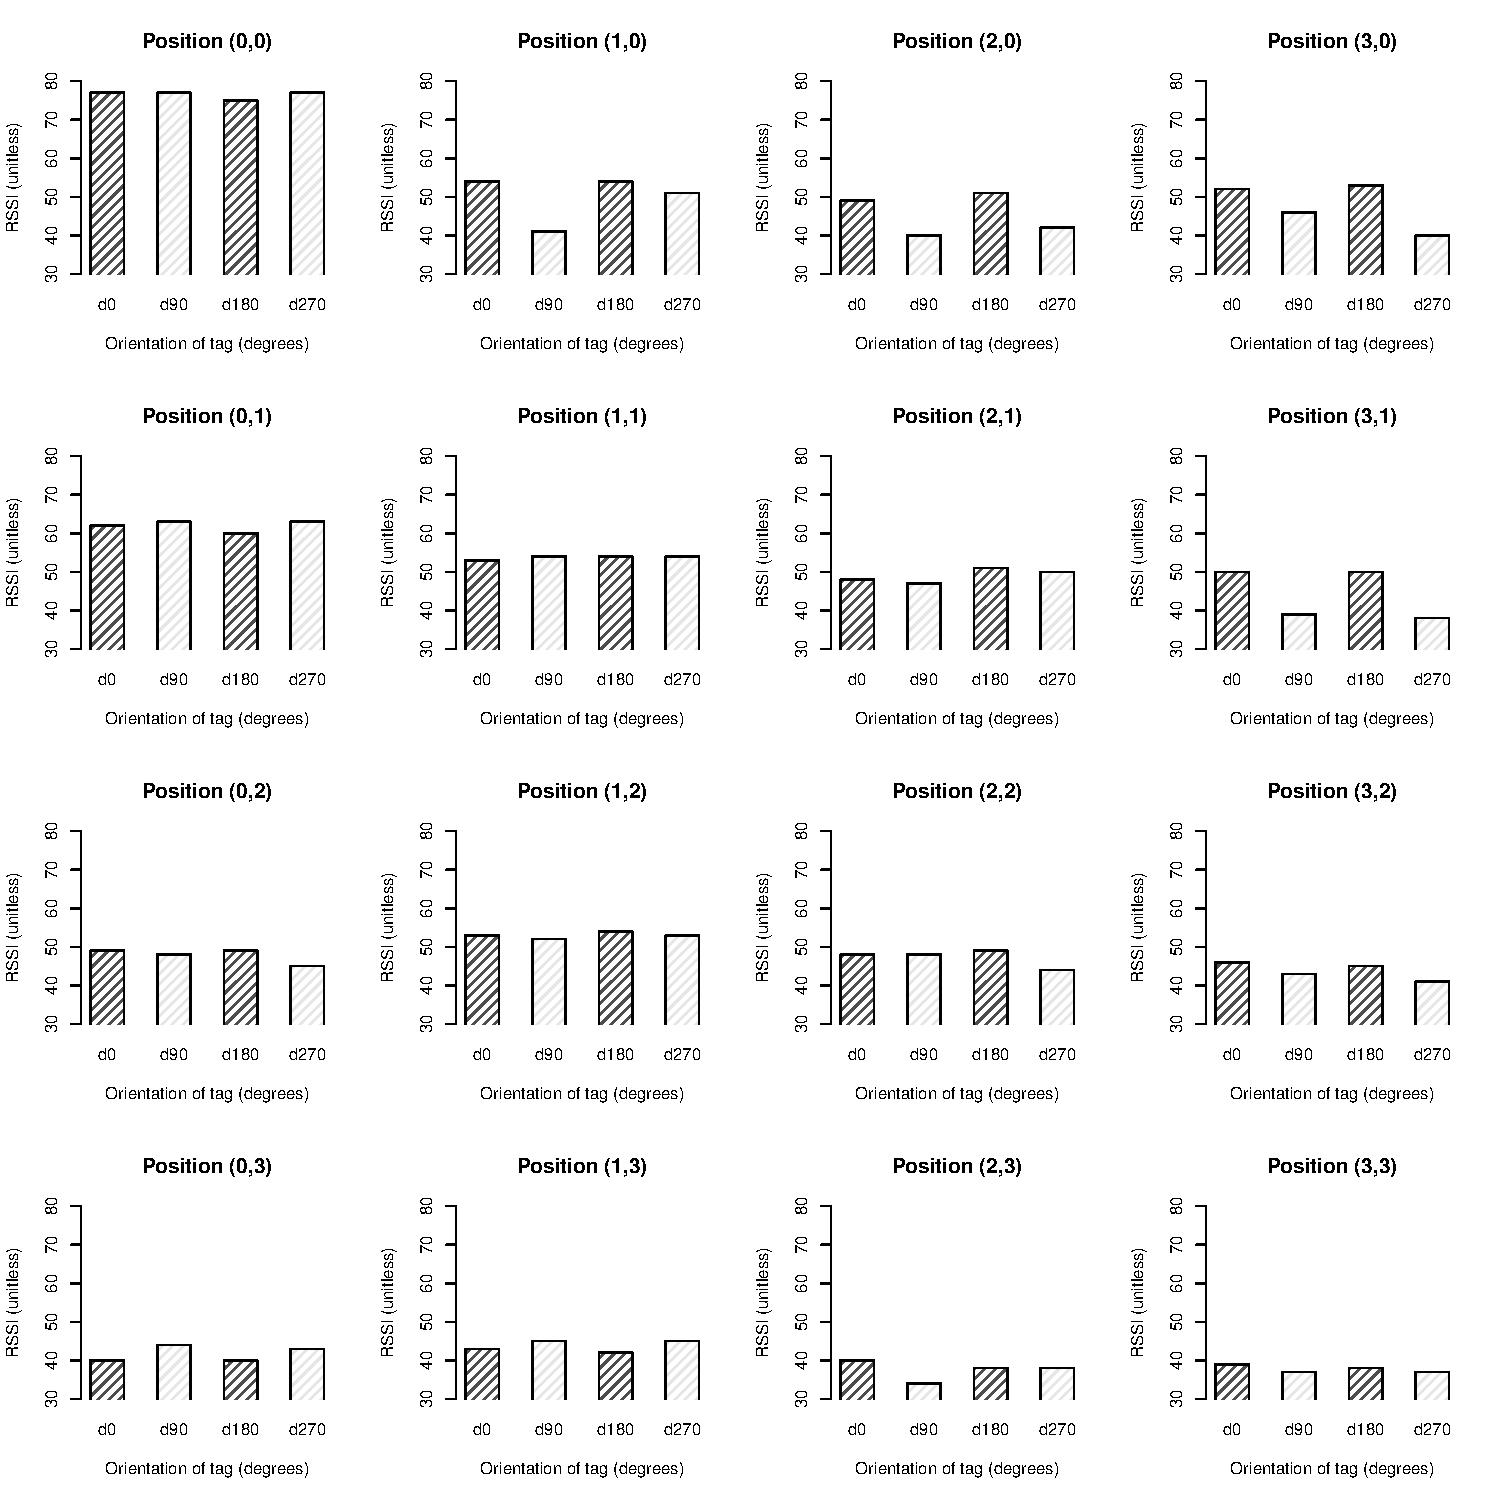
\includegraphics[width=1\textwidth]{figures/rssi_distance_grid_r1}
		\caption{Sixteen plots are organised into a four by four grid. Each plot represents the RSSI measurements of the \textbf{first} reader when the tag is placed at different positions on the x and y axes of the grid. The positions of the tag are all measured in meters. Every four bars in each plot show the RSSI readings when the tag is facing right (0\textdegree), up(90\textdegree), left (180\textdegree), and down (270\textdegree).}
	\end{center}
\end{figure}
\begin{figure}
	\begin{center}
		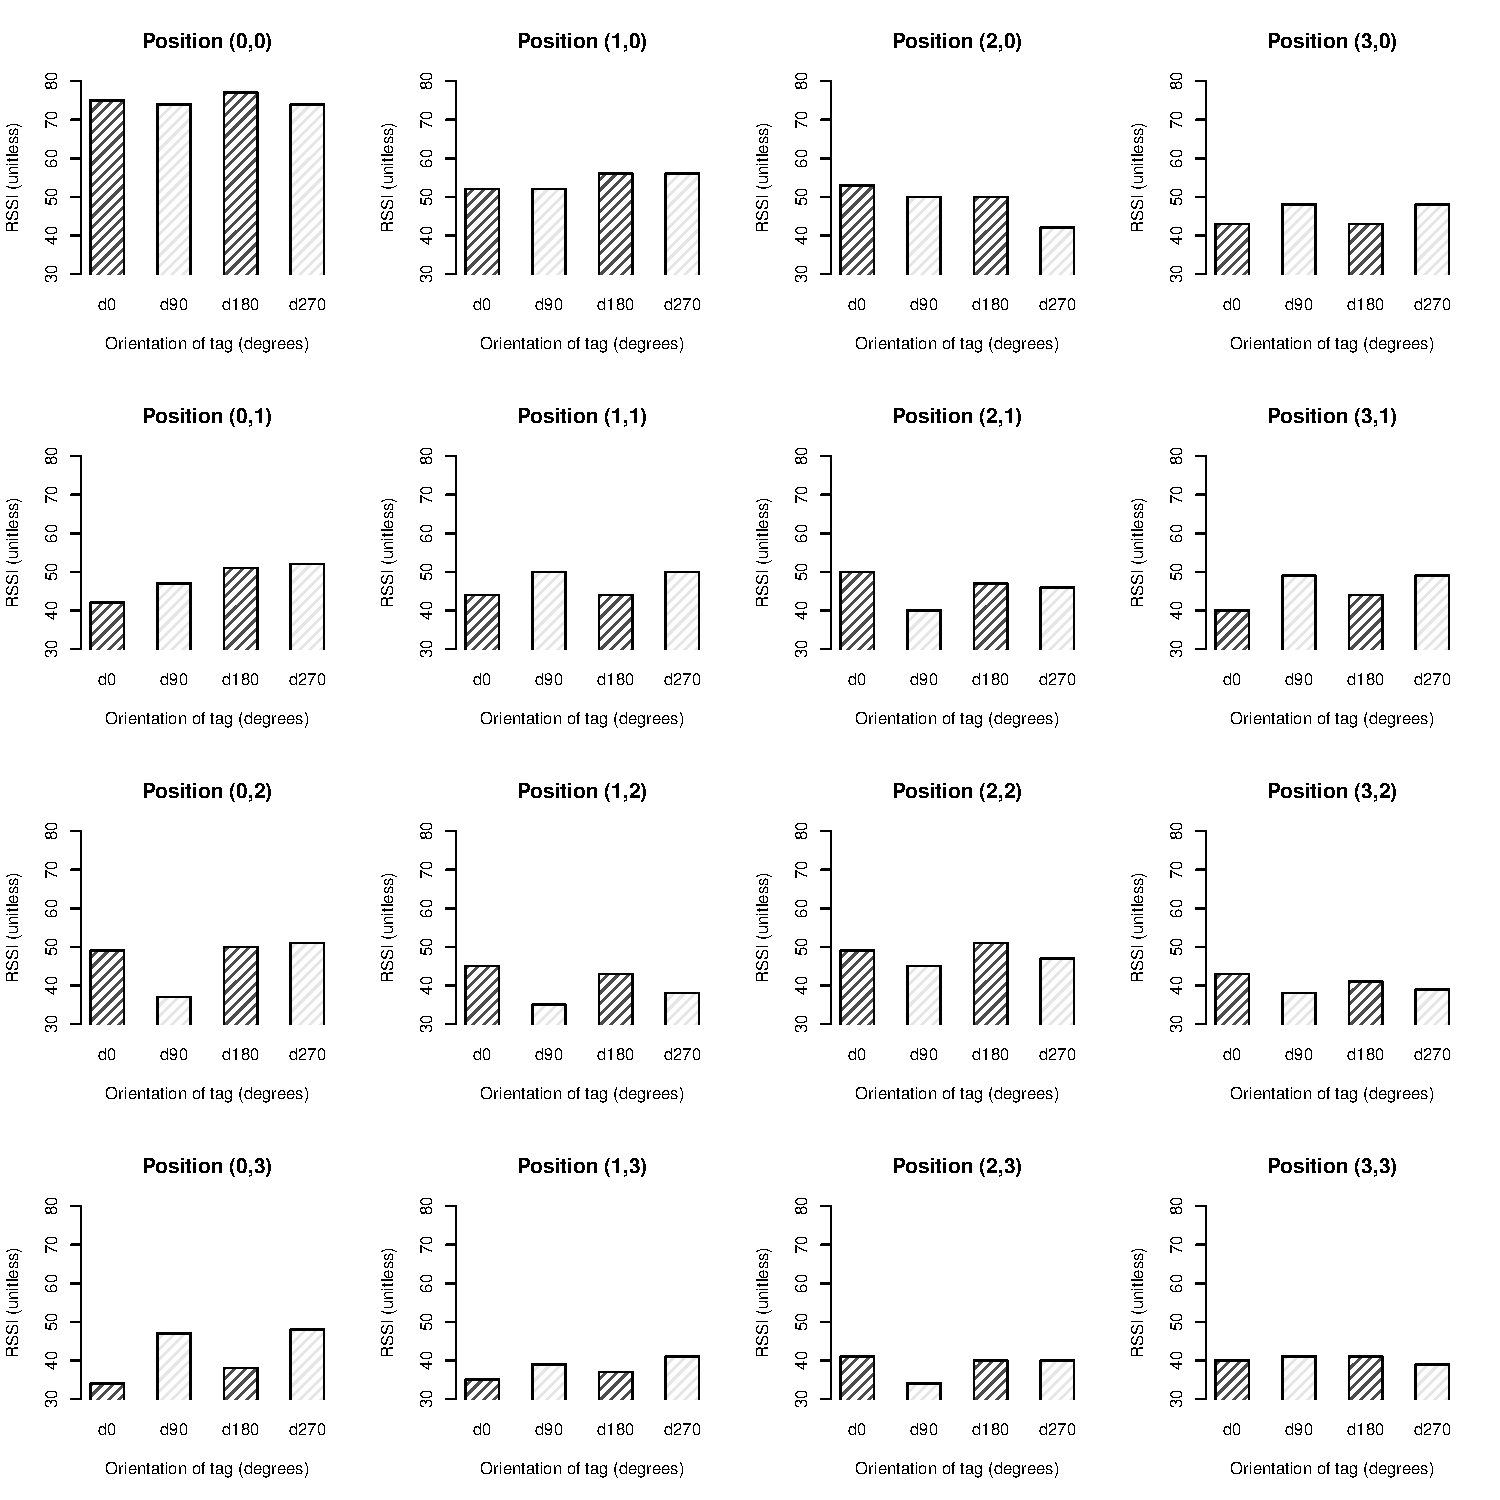
\includegraphics[width=1\textwidth]{figures/rssi_distance_grid_r2}
		\caption{Sixteen plots are organised into a four by four grid. Each plot represents the RSSI measurements of the \textbf{second} reader when the tag is placed at different positions on the x and y axes of the grid. The positions of the tag are all measured in meters. Every four bars in each plot show the RSSI readings when the tag is facing right (0\textdegree), up(90\textdegree), left (180\textdegree), and down (270\textdegree).}
	\end{center}
\end{figure}
\begin{figure}
	\begin{center}
		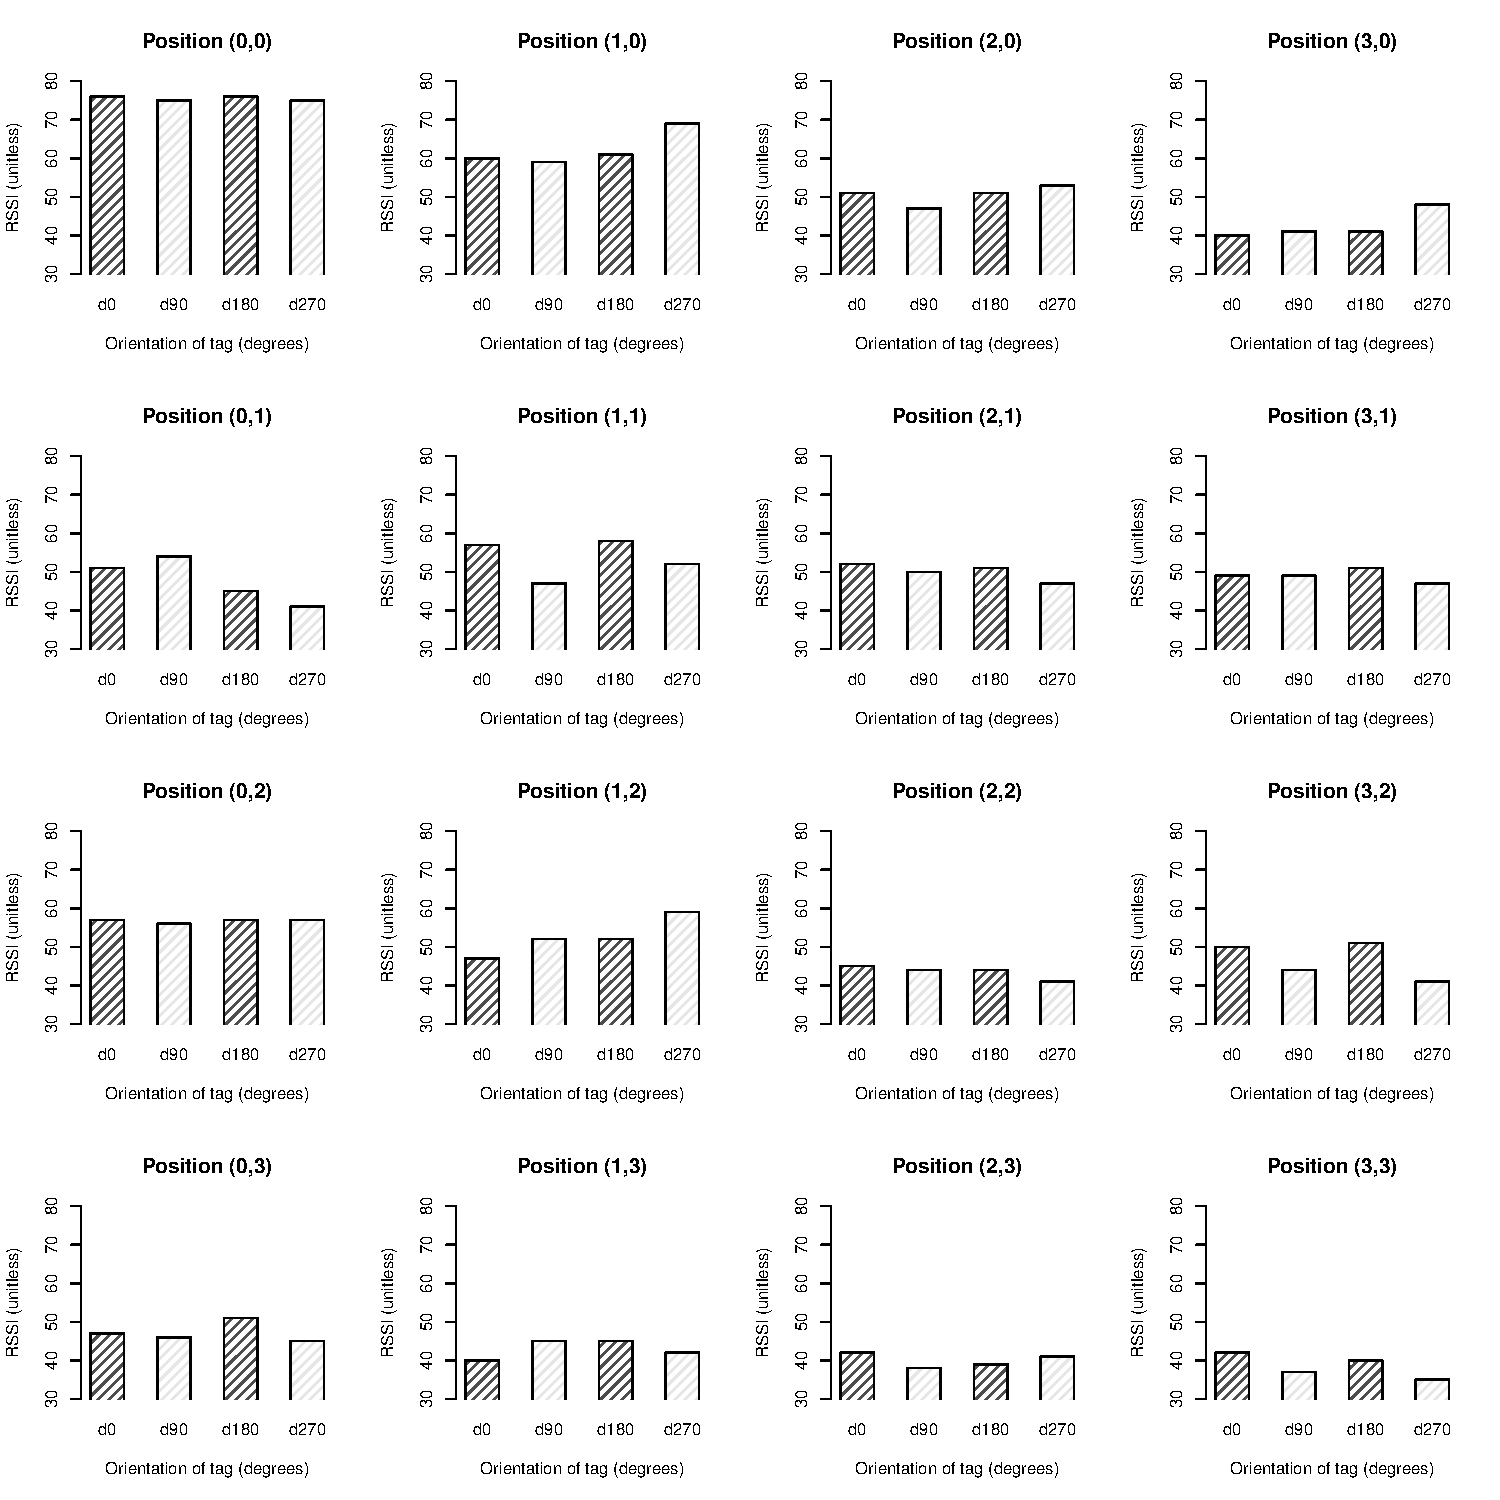
\includegraphics[width=1\textwidth]{figures/rssi_distance_grid_r3}
		\caption{Sixteen plots are organised into a four by four grid. Each plot represents the RSSI measurements of the \textbf{third} reader when the tag is placed at different positions on the x and y axes of the grid. The positions of the tag are all measured in meters. Every four bars in each plot show the RSSI readings when the tag is facing right (0\textdegree), up(90\textdegree), left (180\textdegree), and down (270\textdegree).}
	\end{center}
\end{figure}
\begin{figure}
	\begin{center}
		
\includegraphics[width=1\textwidth]{figures/error_distance_grid}
		\caption{Sixteen plots are organised into a four by four grid. The readers are placed at positions (0,0), (0,3), and (3,0). Each plot represents the error in meters between measured and estimated location when the tag is placed at different positions on the grid. Each plot consists of four ellipses that illustrate the x and y error when the tag is facing right (0\textdegree), up(90\textdegree), left (180\textdegree), and down (270\textdegree). The colours of the ellipses are red, green, blue, and black, respectively.}
	\end{center}
\end{figure}

\begin{figure}
	\begin{center}
		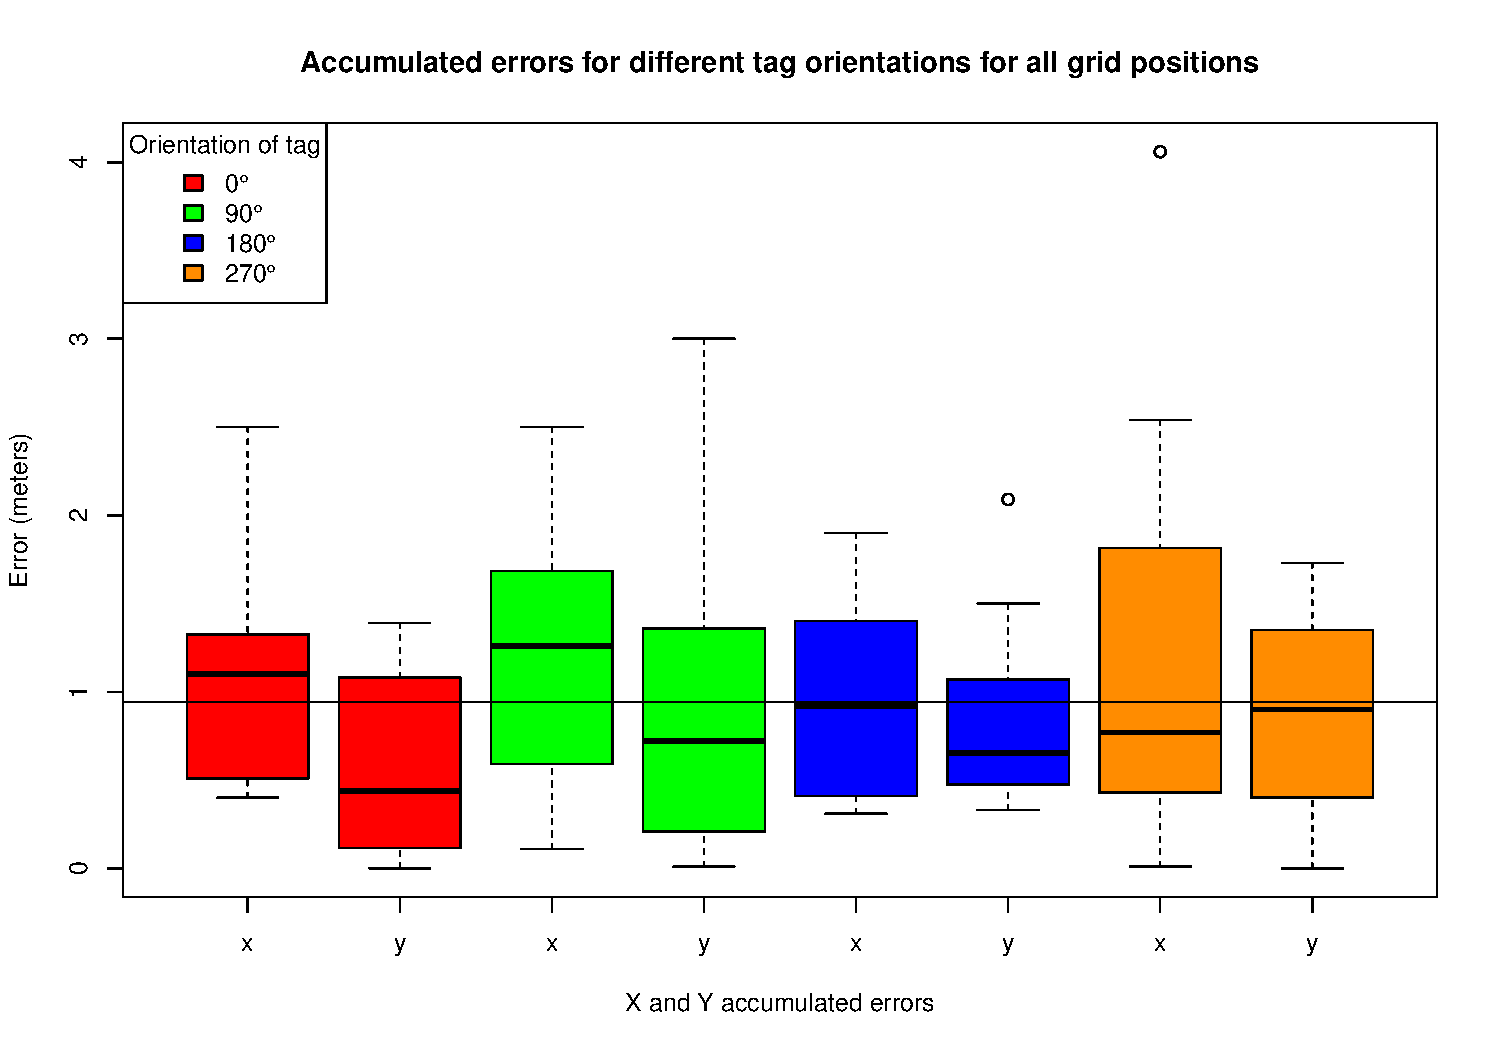
\includegraphics[width=1\textwidth]{figures/error_boxplot}
		\caption{A box plot showing errors between measured and estimated locations. The boxes are organised in four groups. Each group consists of errors in the x and y axes for a particular orientation of the tag. The horizontal line across the plot is the mean of all errors regardless of the tag orientation.}
	\end{center}
\end{figure}

\section{Summary}

\chapter{Discussion}
\label{ch:discussion}

\chapter{Future Work}
\label{ch:future.work}

\chapter{Conclusion}
\label{ch:conclusion}


\appendix
\chapter{Supplementary Information}
\label{ap:appendix}

\section{Hardware setup using Wi-Fi connectivity}
\label{sec:hardsetwifi}

\begin{figure}[h]
	\begin{center}
		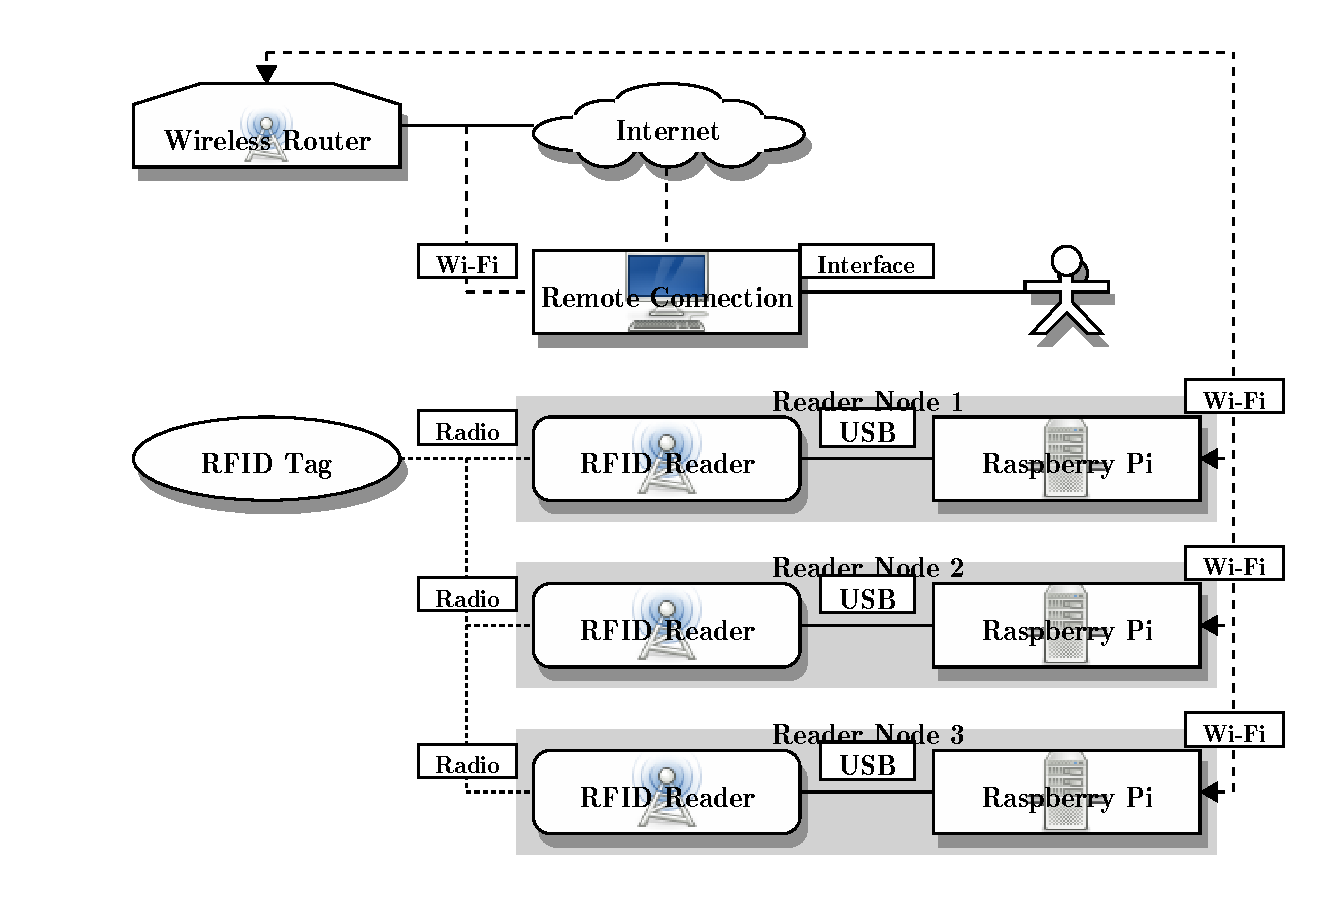
\includegraphics[width=1\textwidth]{figures/blockdiag/hardwaredesignwifi}
		\caption{Hardware setup with wireless connectivity between reader nodes.}
		\label{fig:hardsetwifi}
	\end{center}
\end{figure}

\newpage
\section{Translation tables from RSSI to distance}
\label{sec:trans}

\begin{table}[h]
	\centering
	\begin{tabular}{ | c | c | c || c | c || c | c || c | c || c | c || c | c || c | c | }
		\hline
		Distance 	& 0  & 1  & 1  & 2  & 2  & 3  & 3  & 4  & 4  & 5  & 5  & 6  & 6  & 7  \\ \hline
		RSSI 		& 80 & 65 & 64 & 62 & 61 & 57 & 56 & 53 & 52 & 48 & 47 & 46 & 45 & 44  \\ \hline
	\end{tabular}
	\caption{RSSI value ranges used to estimate distance when using the first reader. }
	\label{tbl:trans1}
\end{table}

\begin{table}[h]
	\centering
	\begin{tabular}{ | c | c | c || c | c || c | c || c | c || c | c || c | c || c | c | }
		\hline
		Distance 	& 0  & 1  & 1  & 2  & 2  & 3  & 3  & 4  & 4  & 5  & 5  & 6  & 6  & 7  \\ \hline
		RSSI 		& 77 & 63 & 62 & 58 & 57 & 55 & 54 &53  & 52 & 49 & 48 & 47 & 46 & 44 \\ \hline
	\end{tabular}
	\caption{RSSI value ranges used to estimate distance when using the second reader. }
	\label{tbl:trans2}
\end{table}

\begin{table}[h]
	\centering
	\begin{tabular}{ | c | c | c || c | c || c | c || c | c || c | c || c | c || c | c | }
		\hline
		Distance 	& 0  & 1  & 1  & 2  & 2  & 3  & 3  & 4  & 4  & 5  & 5  & 6  & 6  & 7  \\ \hline
		RSSI 		& 78 & 64 & 63 & 60 & 59 & 56 & 55 & 54 & 53 & 49 & 48 & 45 & 44 & 43 \\ \hline
	\end{tabular}
	\caption{RSSI value ranges used to estimate distance when using the third reader. }
	\label{tbl:trans3}
\end{table}

\newpage
\section{Orientation of tag to reader}
\label{sec:oriap}

\begin{figure}[H]
	\begin{center}
		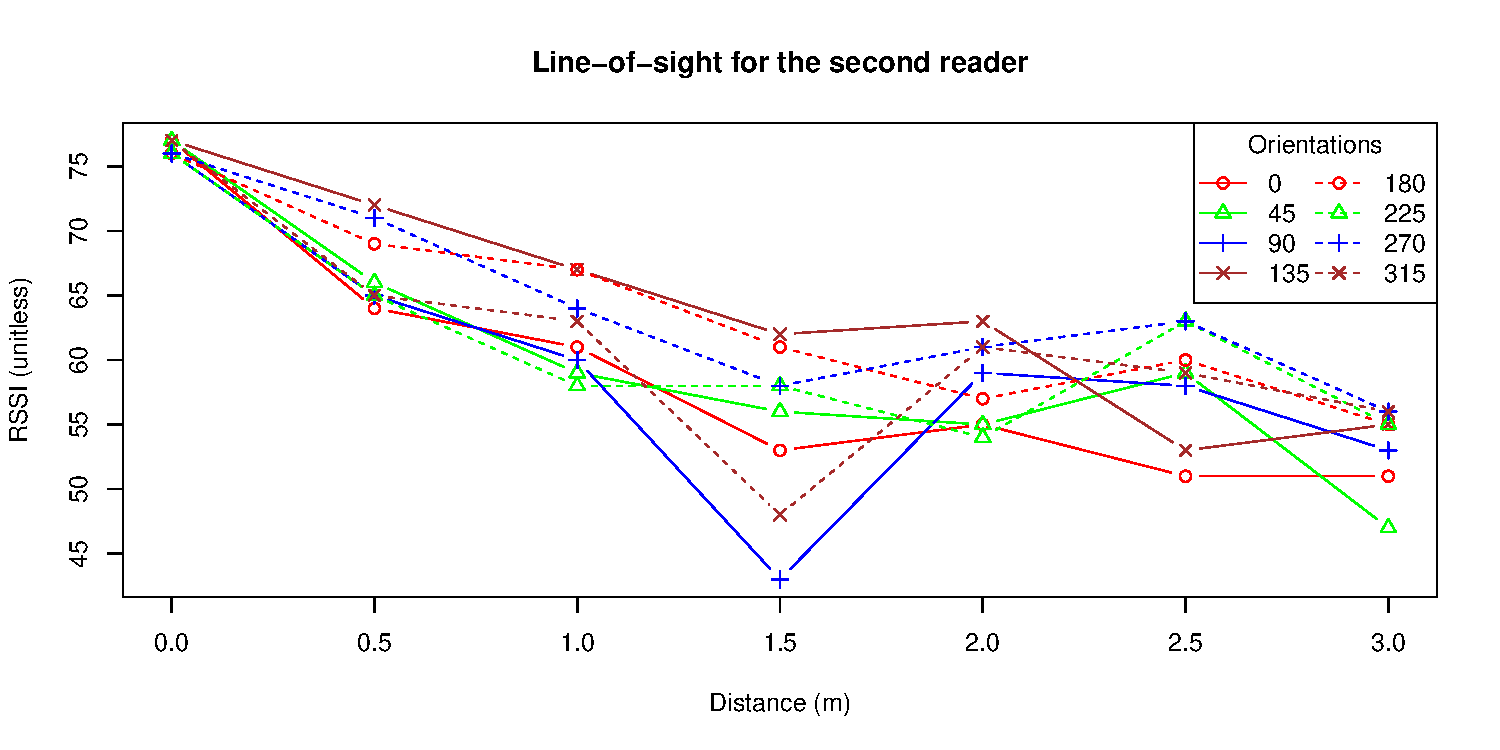
\includegraphics[width=1\textwidth]{figures/rssi_distance_3m_los_r2}
		\caption{Plot of RSSI measurements of different orientations of the tag with respect to the second reader. There was  a line of sight between the RFID devices.}
	\end{center}
\end{figure}

\begin{figure}[H]
	\begin{center}
		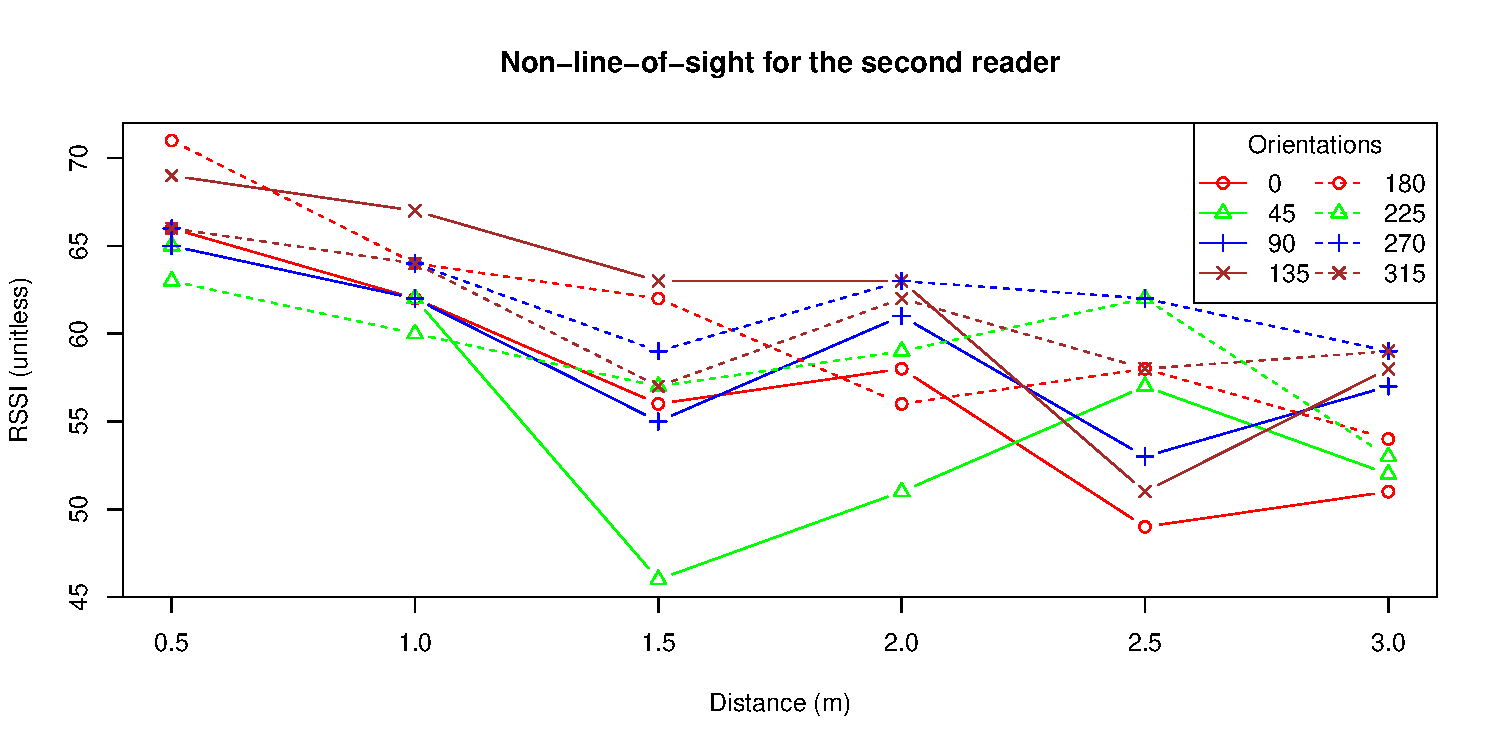
\includegraphics[width=1\textwidth]{figures/rssi_distance_3m_nlos_r2}
		\caption{Plot of RSSI measurements of different orientations of the tag with respect to the second reader. The tag was obscured by an object.}
	\end{center}
\end{figure}

\begin{figure}[H]
	\begin{center}
		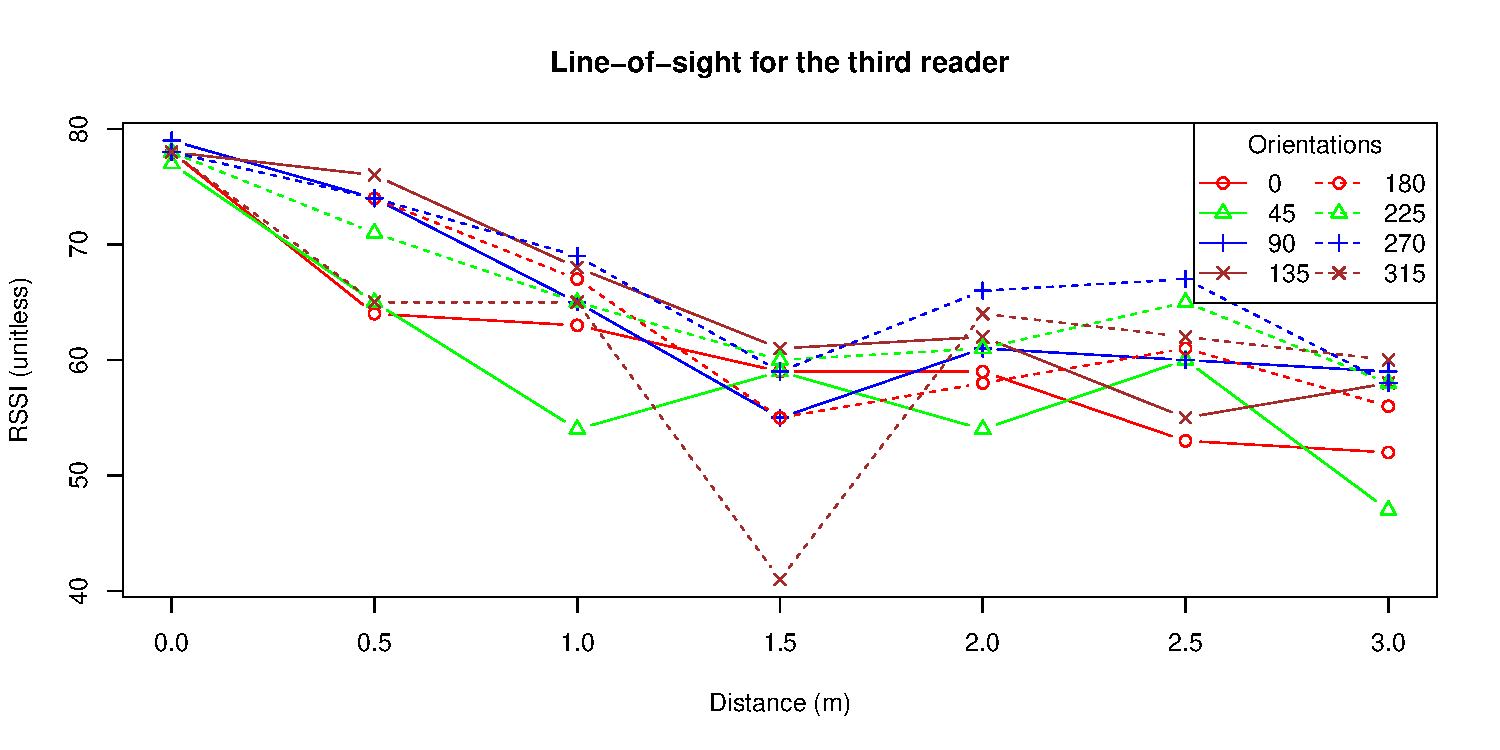
\includegraphics[width=1\textwidth]{figures/rssi_distance_3m_los_r3}
		\caption{Plot of RSSI measurements of different orientations of the tag with respect to the third reader. There was  a line of sight between the RFID devices.}
	\end{center}
\end{figure}

\begin{figure}[H]
	\begin{center}
		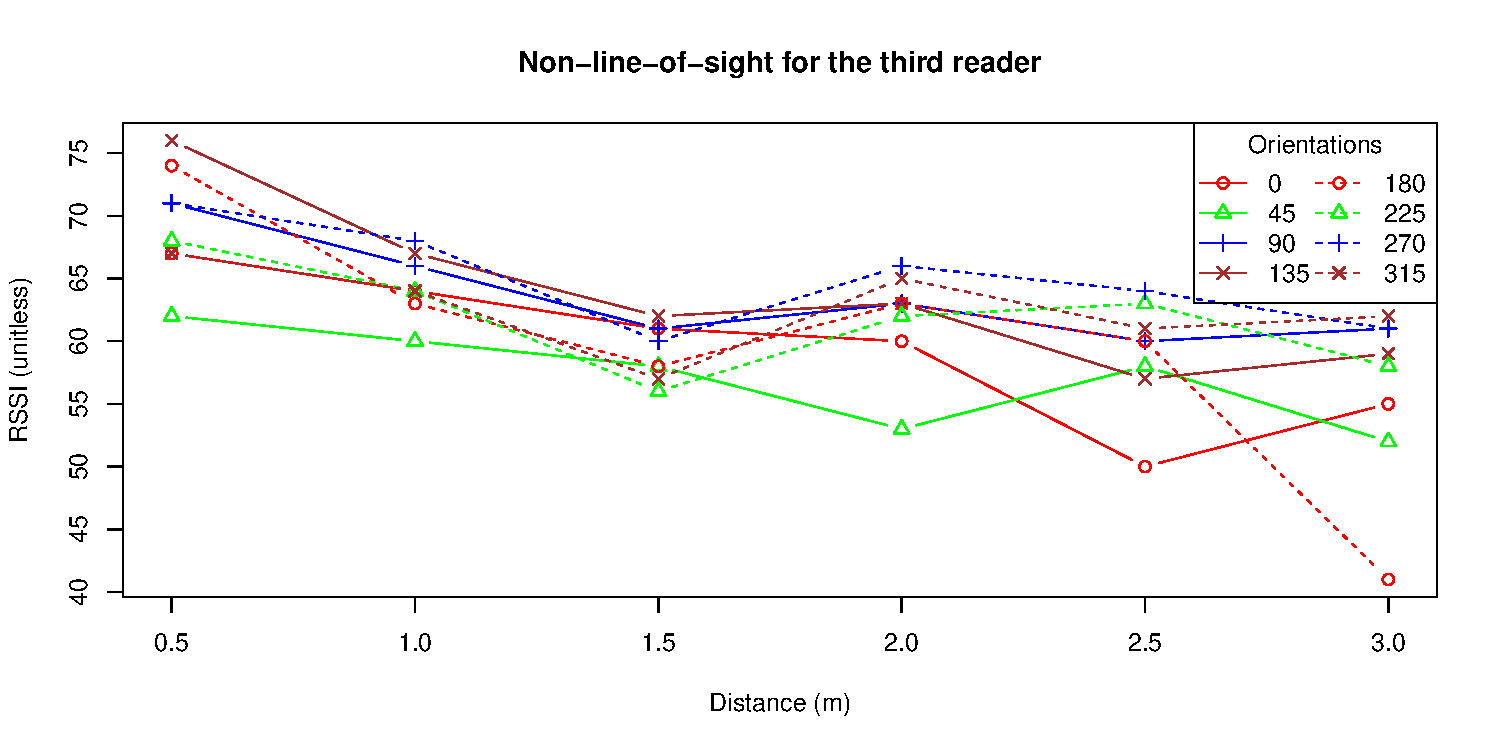
\includegraphics[width=1\textwidth]{figures/rssi_distance_3m_nlos_r3}
		\caption{Plot of RSSI measurements of different orientations of the tag with respect to the third reader. The tag was obscured by an object.}
	\end{center}
\end{figure}

\begin{figure}[H]
	\begin{center}
		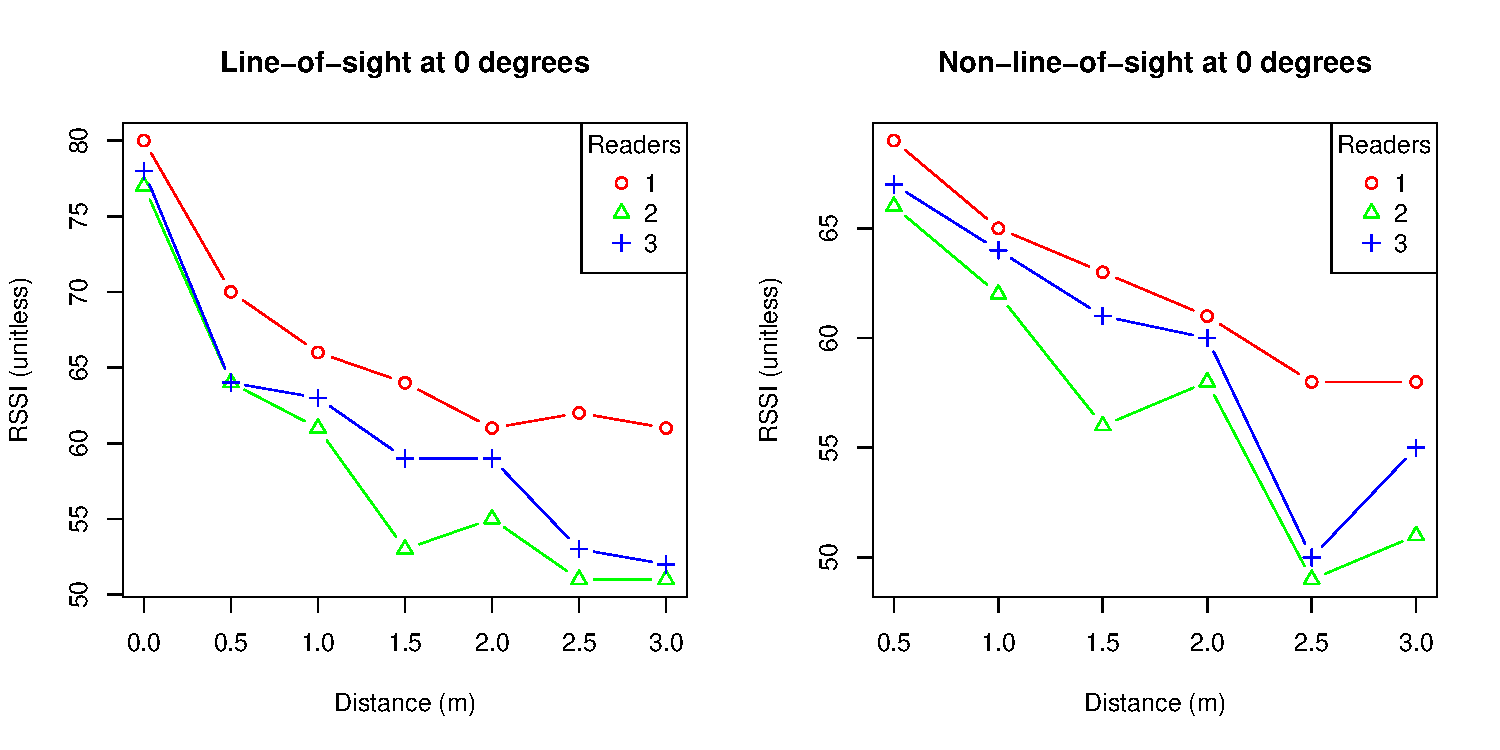
\includegraphics[width=1\textwidth]{figures/rssi_distance_3m_0deg}
		\caption{Two plots of RSSI measurements at increasing distances with the readers at 0 degrees (antennas facing the tag). The left graph show how RSSI values change with a line-of-sight signal propagation. The right graph illustrates the same experiment but with a non-line-of-sight signal propagation (there is an obstacle between the reader and the tag).}
	\end{center}
\end{figure}

\begin{figure}[H]
	\begin{center}
		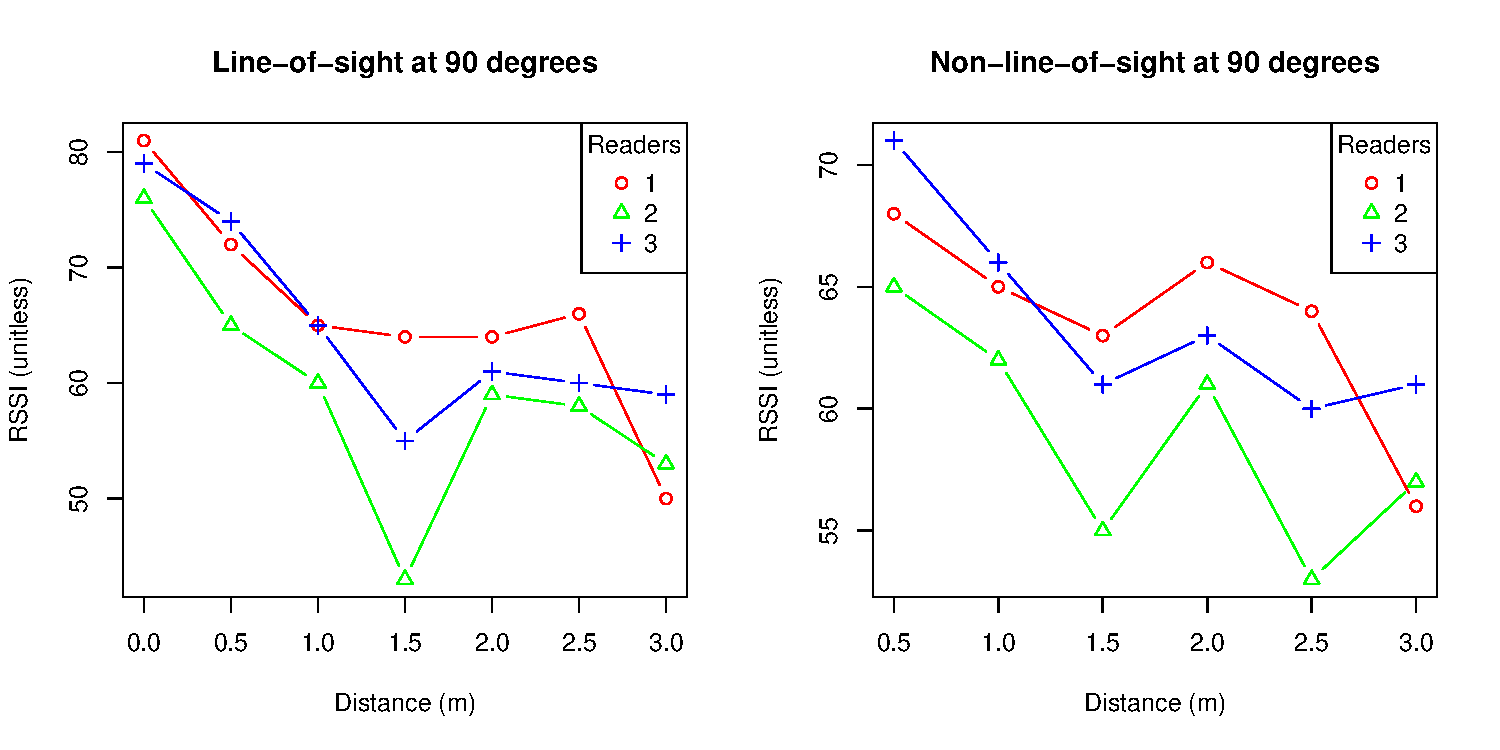
\includegraphics[width=1\textwidth]{figures/rssi_distance_3m_90deg}
		\caption{Two plots of RSSI measurements at increasing distances with the readers at 90 degrees (antennas at an angle to the tag). The left graph show how RSSI values change with a line-of-sight signal propagation. The right graph illustrates the same experiment but with a non-line-of-sight signal propagation (there is an obstacle between the reader and the tag).}
	\end{center}
\end{figure}

\begin{figure}[H]
	\begin{center}
		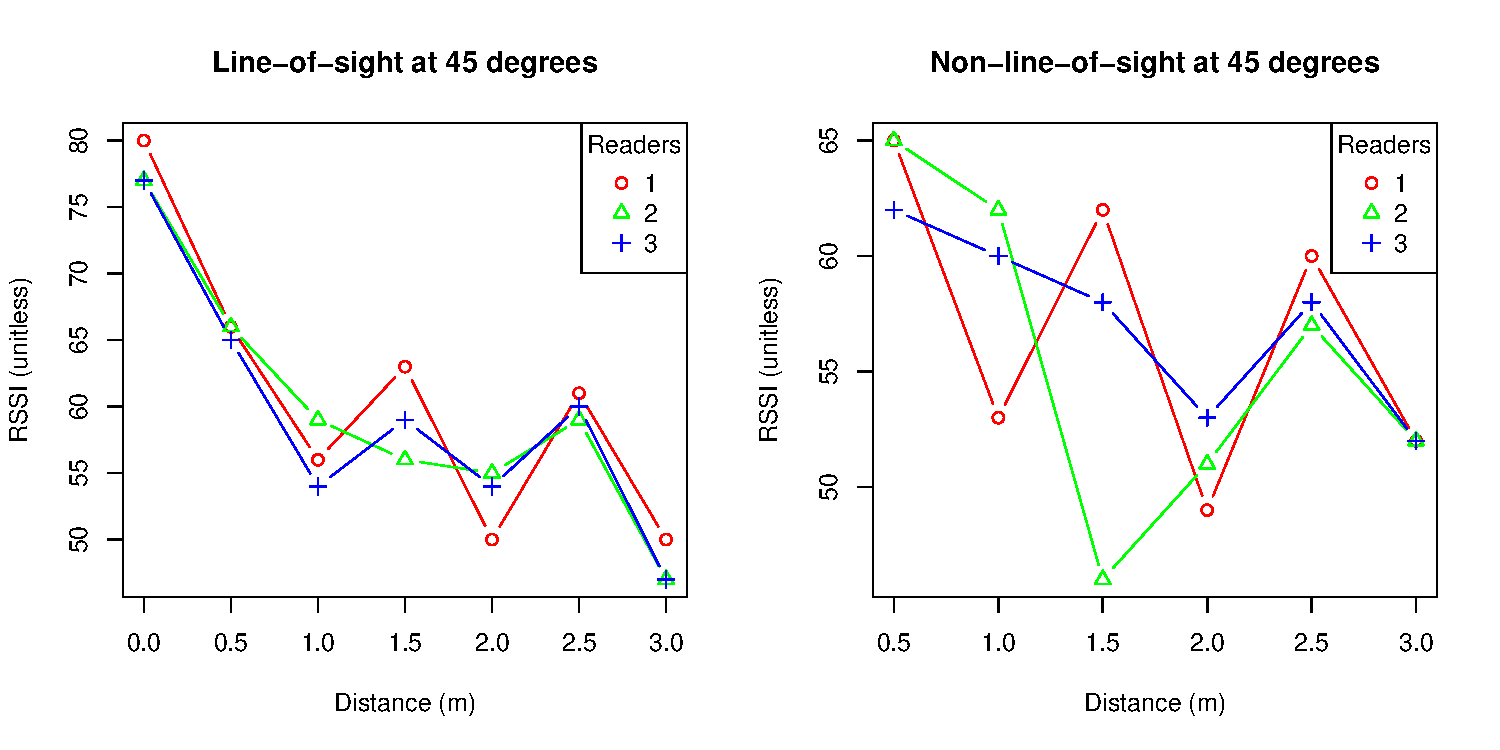
\includegraphics[width=1\textwidth]{figures/rssi_distance_3m_45deg}
		\caption{Two plots of RSSI measurements at increasing distances with the readers at 45 degrees (antennas at an angle to the tag). The left graph show how RSSI values change with a line-of-sight signal propagation. The right graph illustrates the same experiment but with a non-line-of-sight signal propagation (there is an obstacle between the reader and the tag).}
	\end{center}
\end{figure}

\begin{figure}[H]
	\begin{center}
		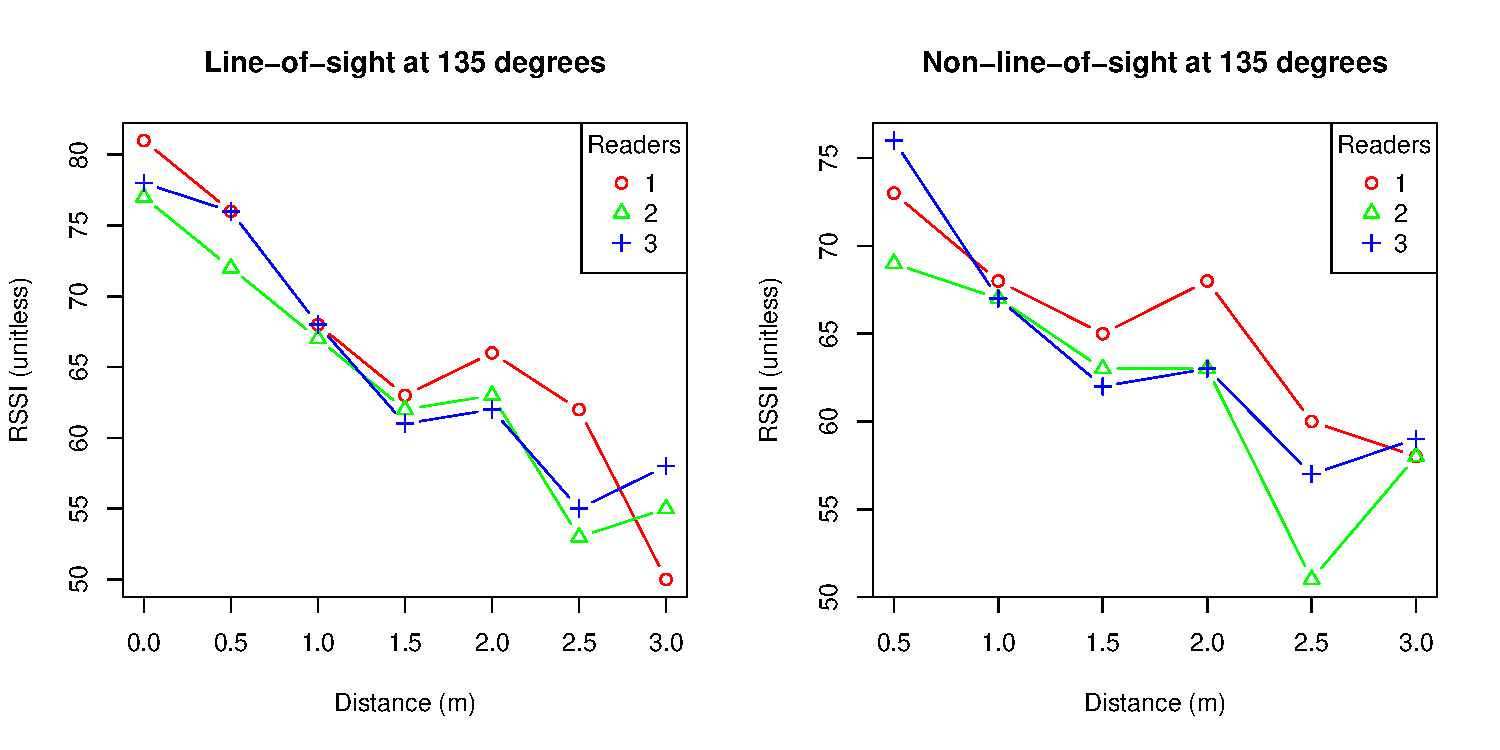
\includegraphics[width=1\textwidth]{figures/rssi_distance_3m_135deg}
		\caption{Two plots of RSSI measurements at increasing distances with the readers at 135 degrees (antennas at an angle to the tag). The left graph show how RSSI values change with a line-of-sight signal propagation. The right graph illustrates the same experiment but with a non-line-of-sight signal propagation (there is an obstacle between the reader and the tag).}
	\end{center}
\end{figure}

\begin{figure}[H]
	\begin{center}
		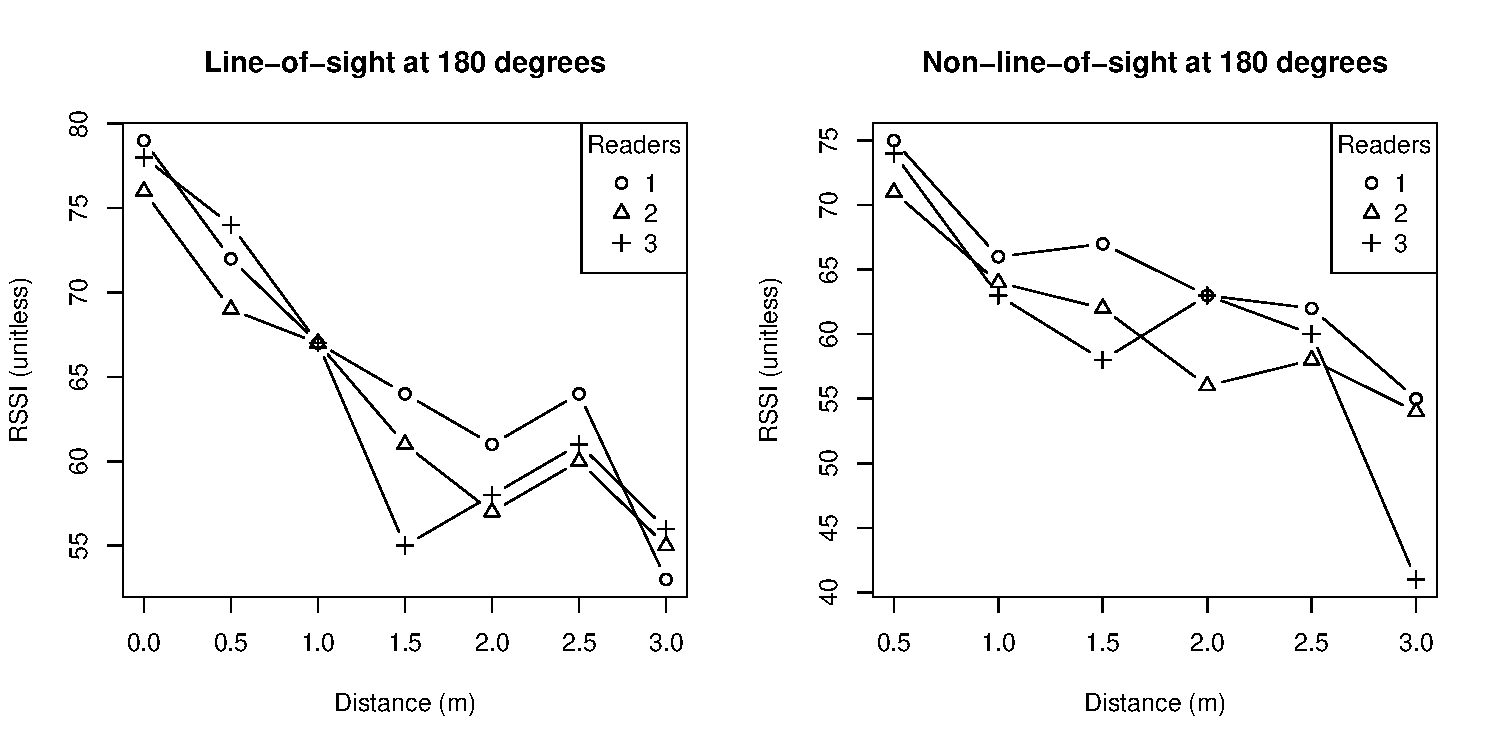
\includegraphics[width=1\textwidth]{figures/rssi_distance_3m_180deg}
		\caption{Two plots of RSSI measurements at increasing distances with the readers at 180 degrees (antennas at an angle to the tag). The left graph show how RSSI values change with a line-of-sight signal propagation. The right graph illustrates the same experiment but with a non-line-of-sight signal propagation (there is an obstacle between the reader and the tag).}
	\end{center}
\end{figure}

\begin{figure}[H]
	\begin{center}
		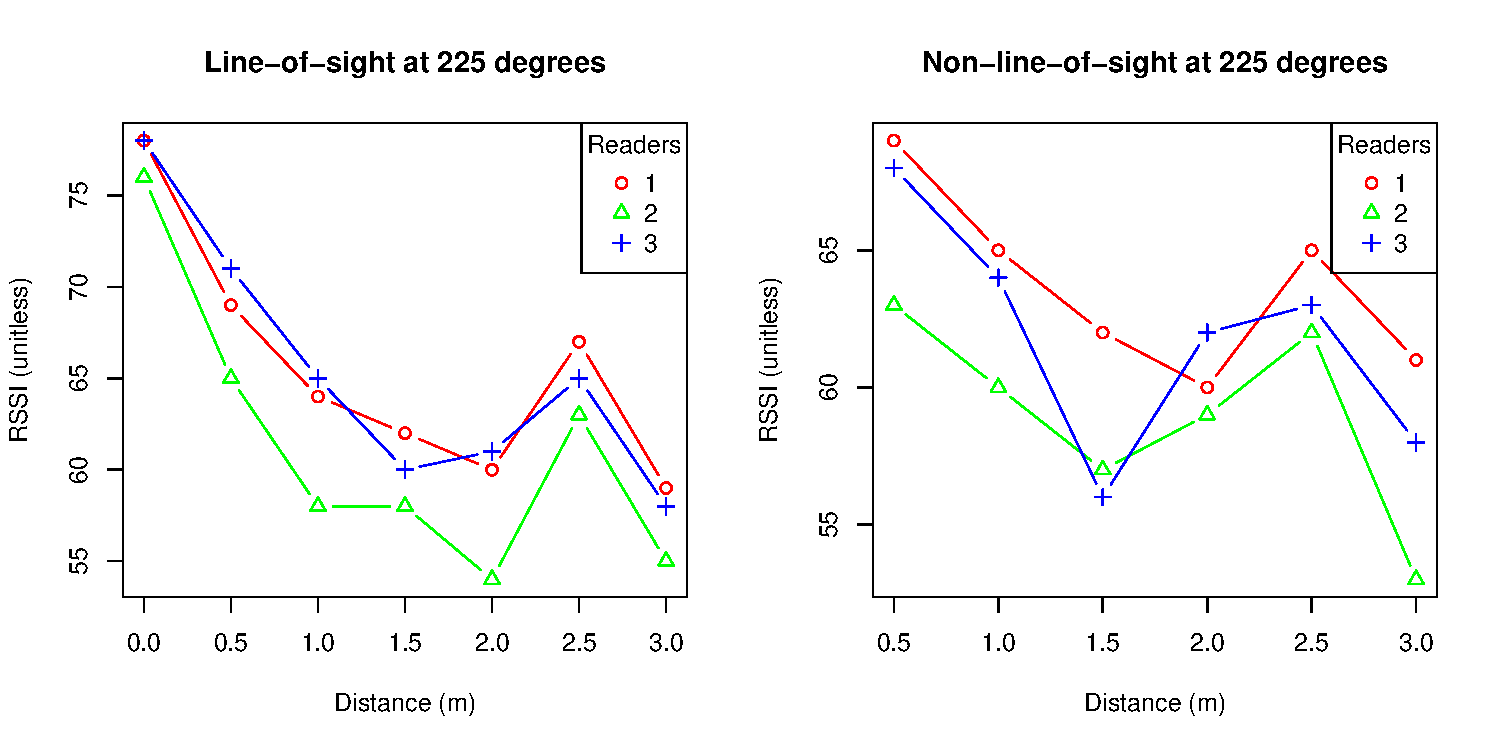
\includegraphics[width=1\textwidth]{figures/rssi_distance_3m_225deg}
		\caption{Two plots of RSSI measurements at increasing distances with the readers at 225 degrees (antennas at an angle to the tag). The left graph show how RSSI values change with a line-of-sight signal propagation. The right graph illustrates the same experiment but with a non-line-of-sight signal propagation (there is an obstacle between the reader and the tag).}
	\end{center}
\end{figure}

\begin{figure}[H]
	\begin{center}
		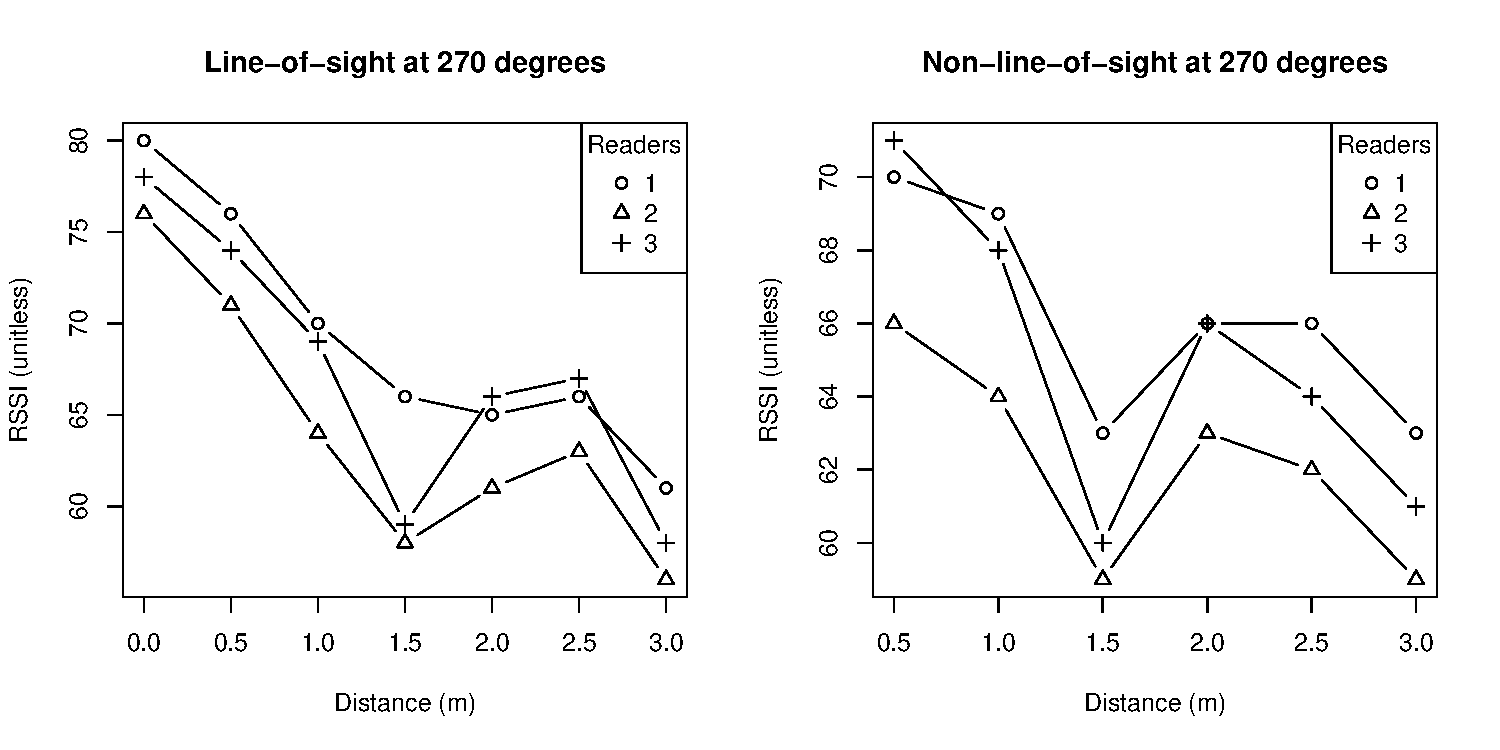
\includegraphics[width=1\textwidth]{figures/rssi_distance_3m_270deg}
		\caption{Two plots of RSSI measurements at increasing distances with the readers at 270 degrees (antennas at an angle to the tag). The left graph show how RSSI values change with a line-of-sight signal propagation. The right graph illustrates the same experiment but with a non-line-of-sight signal propagation (there is an obstacle between the reader and the tag).}
	\end{center}
\end{figure}

\begin{figure}[H]
	\begin{center}
		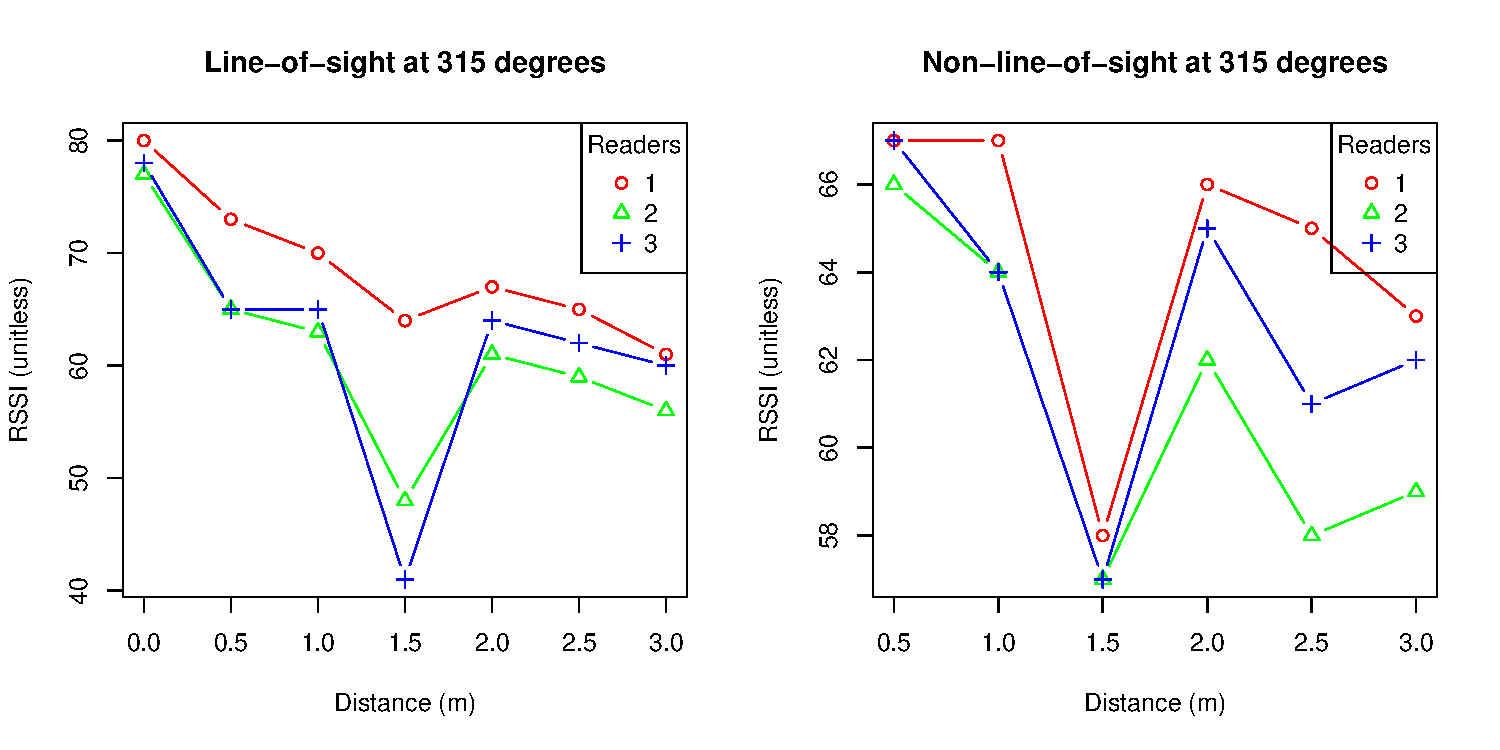
\includegraphics[width=1\textwidth]{figures/rssi_distance_3m_315deg}
		\caption{Two plots of RSSI measurements at increasing distances with the readers at 315 degrees (antennas at an angle to the tag). The left graph show how RSSI values change with a line-of-sight signal propagation. The right graph illustrates the same experiment but with a non-line-of-sight signal propagation (there is an obstacle between the reader and the tag).}
	\end{center}
\end{figure}

\newpage
\section{Grid}

\begin{figure}[H]
	\begin{center}
		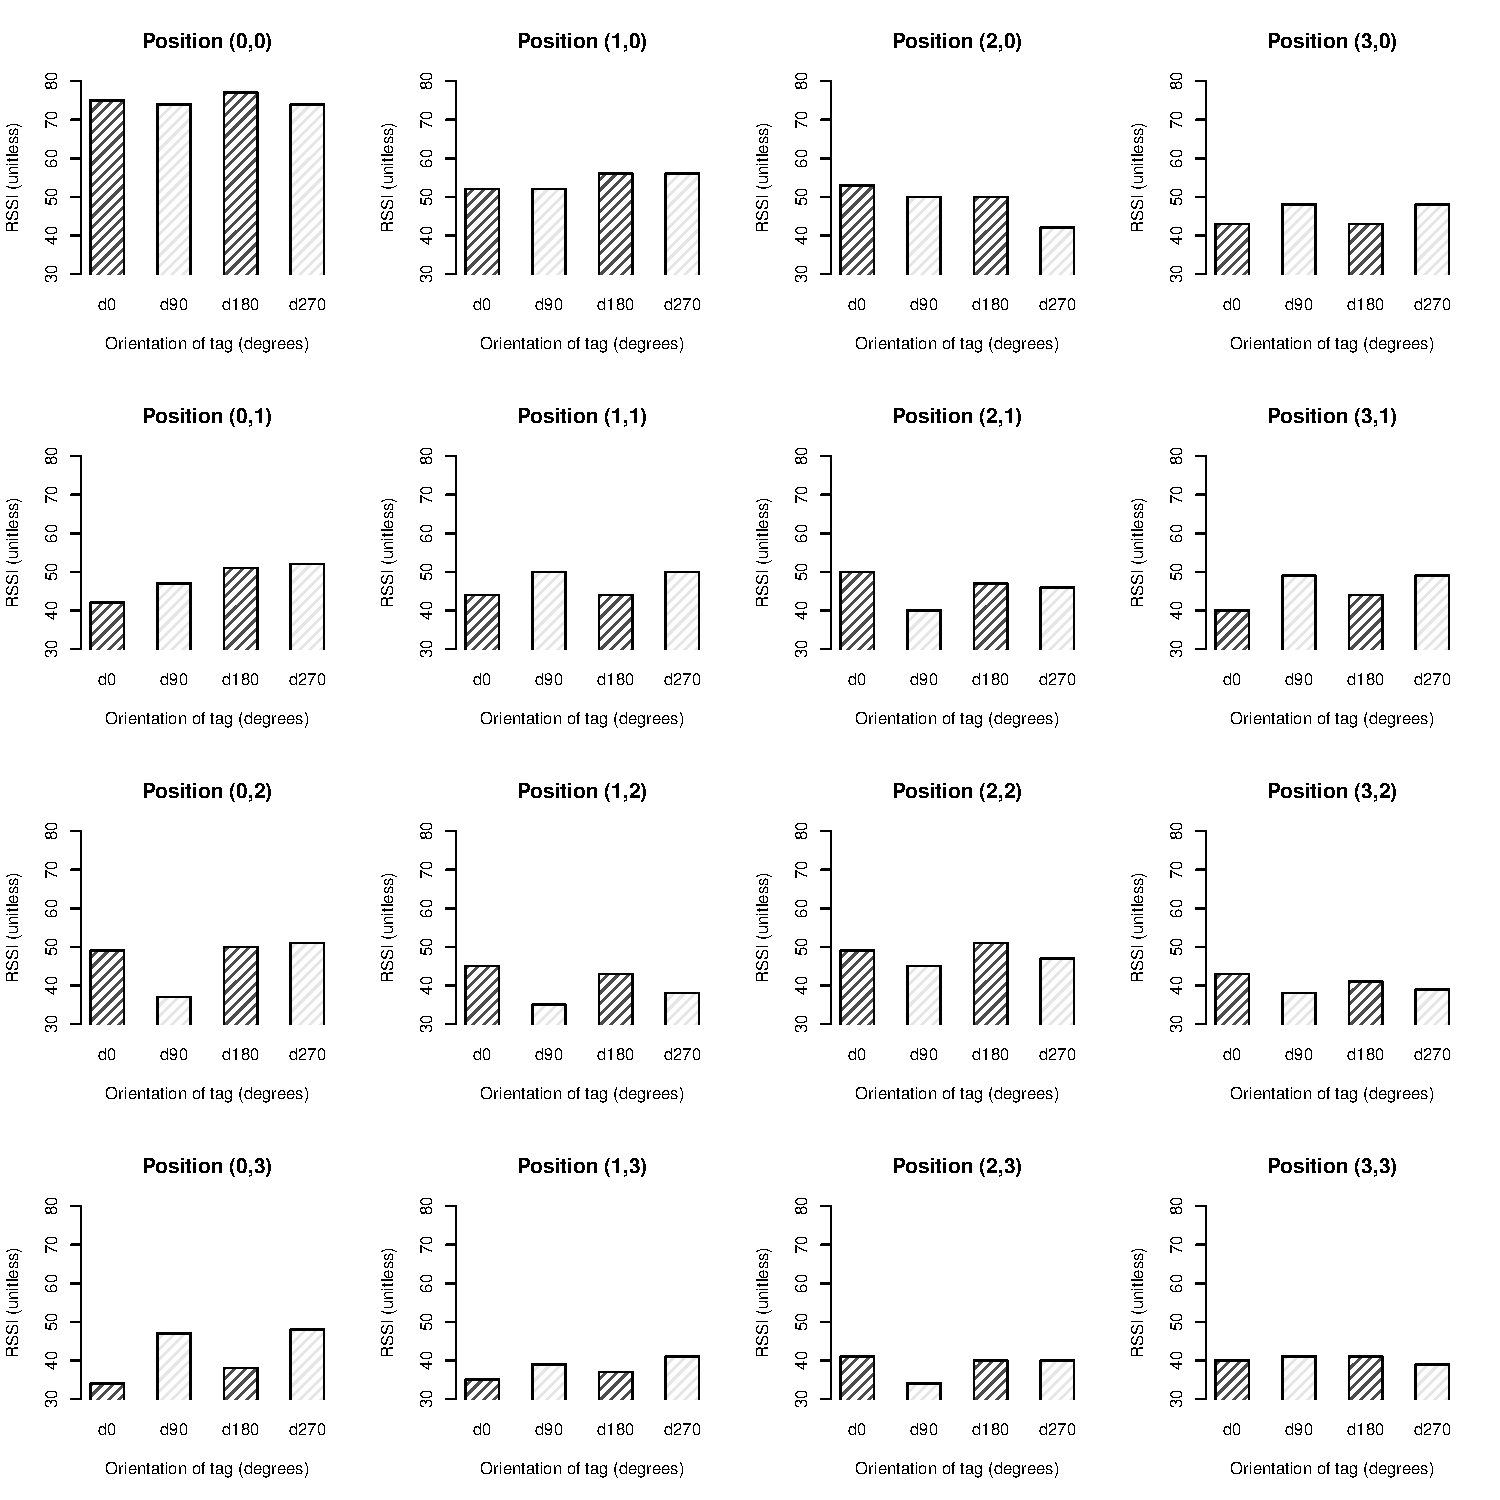
\includegraphics[width=1\textwidth]{figures/rssi_distance_grid_r2}
		\caption{Sixteen plots are organised into a four by four grid. Each plot represents the RSSI measurements of the \textbf{second} reader when the tag is placed at different positions on the x and y axes of the grid. The positions of the tag are all measured in meters. Every four bars in each plot show the RSSI readings when the tag is facing right (0\textdegree), up(90\textdegree), left (180\textdegree), and down (270\textdegree).}
	\end{center}
\end{figure}

\begin{figure}[H]
	\begin{center}
		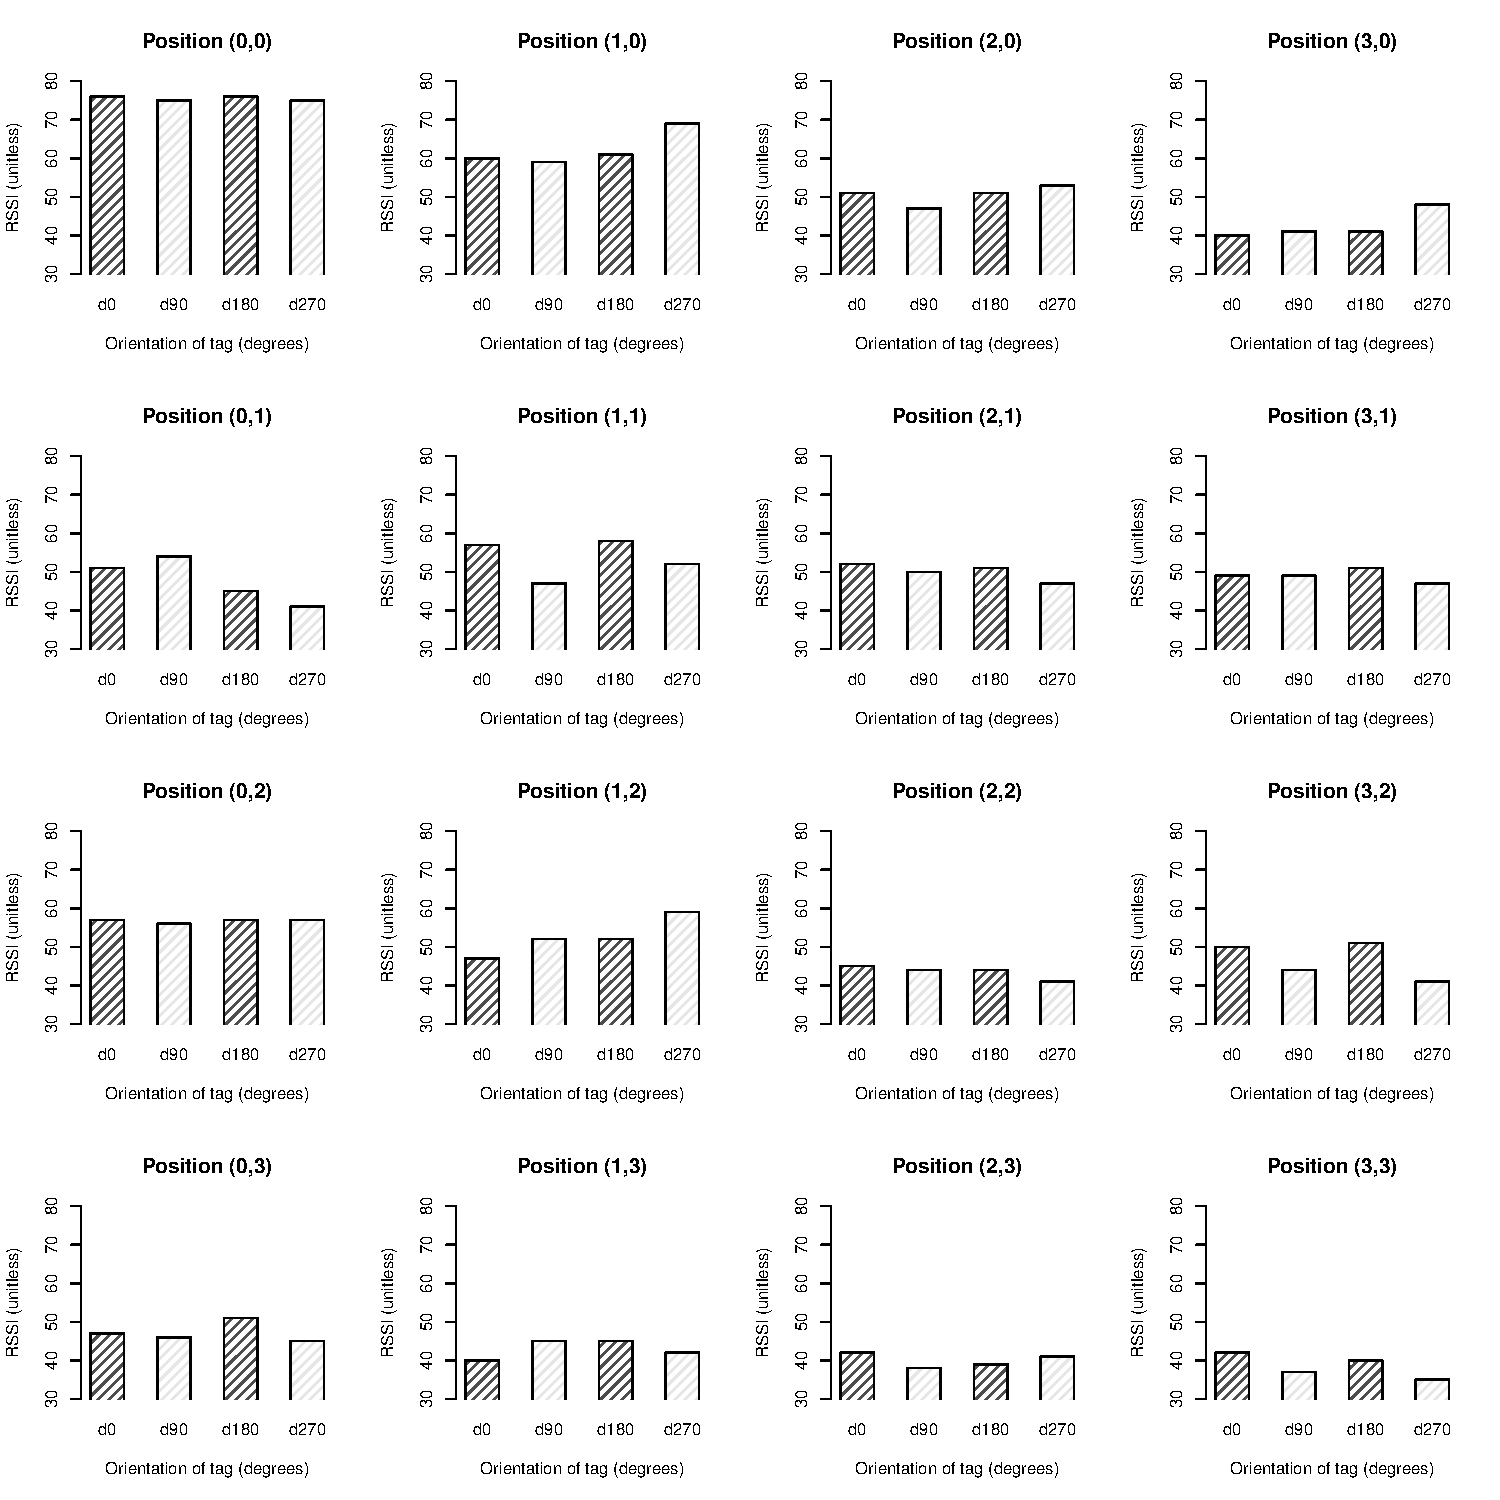
\includegraphics[width=1\textwidth]{figures/rssi_distance_grid_r3}
		\caption{Sixteen plots are organised into a four by four grid. Each plot represents the RSSI measurements of the \textbf{third} reader when the tag is placed at different positions on the x and y axes of the grid. The positions of the tag are all measured in meters. Every four bars in each plot show the RSSI readings when the tag is facing right (0\textdegree), up(90\textdegree), left (180\textdegree), and down (270\textdegree).}
	\end{center}
\end{figure}


\bibliographystyle{apalike}
\bibliography{../library}

\end{document}
